\documentclass[usenames,dvipsnames]{beamer}
\usepackage[utf8]{inputenc} % allow utf-8 input
\usepackage[T1]{fontenc}    % use 8-bit T1 fonts
\usepackage{hyperref}       % hyperlinks
\usepackage{url}            % simple URL typesetting
\usepackage{booktabs}       % professional-quality tables
\usepackage{amsfonts}       % blackboard math symbols
\usepackage{nicefrac}       % compact symbols for 1/2, etc.
\usepackage{microtype}      % microtypography
\usepackage{amsmath}
\usepackage{mathtools}
\usepackage{tikz}
\usetikzlibrary{calc}
\usetikzlibrary{bayesnet}
\usetikzlibrary{arrows}
\usepackage{color}
\usepackage{array}
\usepackage{dsfont}
\usepackage{multirow, graphicx}
 \usepackage{float}
\newcolumntype{C}[1]{>{\centering\arraybackslash}p{#1}}
\newcolumntype{R}[1]{>{\raggedleft\arraybackslash}p{#1}}
\newcolumntype{L}[1]{>{\raggedright\arraybackslash}p{#1}}
\usepackage{caption}
\usepackage{subfig}
\usepackage{pifont}
\usepackage{xcolor}
\usepackage{algorithm,algorithmic}
% \floatname{algorithm}{Procedure}
\renewcommand{\algorithmicrequire}{\textbf{Input:}}
\renewcommand{\algorithmicensure}{\textbf{Output:}}
\newcommand{\cmark}{\textcolor{green!80!black}{\ding{51}}}
\newcommand{\xmark}{\textcolor{red}{\ding{55}}}
\DeclareMathOperator*{\argmin}{argmin}
\urlstyle{same}
\usepackage{listings}
\usepackage[export]{adjustbox}
\usepackage{inconsolata}
% \usetheme{Boadilla}

\title{Attention is All You Need}
% \subtitle{Using Beamer}
\author{Bill Watson}
\institute{S\&P Global}
\date{\today}

\newenvironment{nospaceflalign*}
 {\setlength{\abovedisplayskip}{0pt}\setlength{\belowdisplayskip}{0pt}%
  \csname flalign*\endcsname}
 {\csname endflalign*\endcsname\ignorespacesafterend}

\AtBeginSection[]{
  \begin{frame}
  \vfill
  \centering
  \begin{beamercolorbox}[sep=8pt,center,shadow=true,rounded=true]{title}
    \usebeamerfont{title}\insertsectionhead\par%
  \end{beamercolorbox}
  \vfill
  \end{frame}
}

\begin{document}

\begin{frame}
\titlepage
\end{frame}


\begin{frame}
\frametitle{Recap: Encoder-Decoder Models}
\begin{figure}
  \centering
  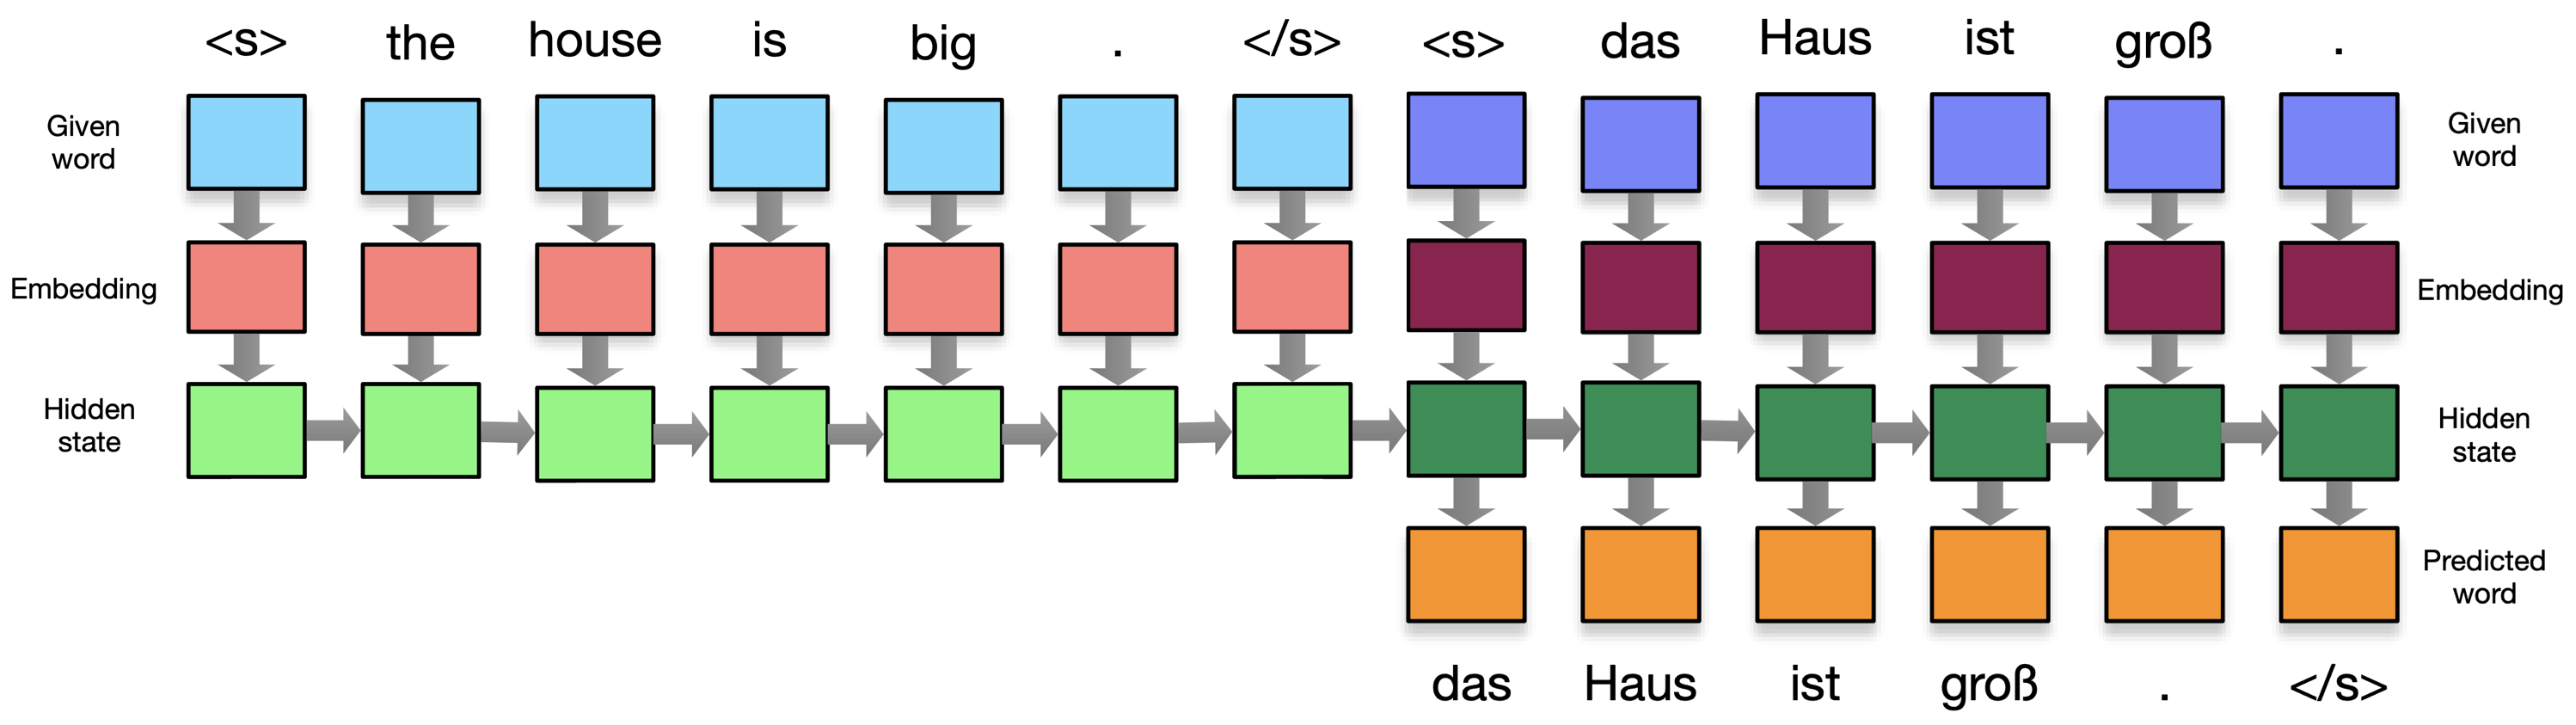
\includegraphics[width=10cm, valign=c]{assets/enc-dec}
\end{figure}
\begin{itemize}
  \item \textbf{Encoders:} Give the source sentence meaning
  \item \textbf{Decoders:} Emit a variable-length sequence
  \item \textbf{Seq2Seq} models rely on propagating the hidden state for generation
\end{itemize}
\end{frame}

\begin{frame}
\frametitle{How can we improve this model?}
\begin{itemize}
  \item Add an \textbf{alignment model} to force the model to 'attend' and 'read' different parts of the input
  \item Gives the decoder direct access to the encodings to make generations
  \item Known as a \textbf{context vector}
\end{itemize}
\end{frame}

\begin{frame}
\frametitle{What are Context Vectors?}
\begin{equation*}
  c_i = \sum_{j} \alpha_{ij} \cdot h_j
\end{equation*}
\begin{itemize}
  \item A \textbf{context vector} $c_i$ is the weighted sum of the encodings for the $i$-th iteration of the decoder
  \item $s_{i-1}$ is the previous hidden state of the decoder
  \item $h_j$ is the encoding for the $j$-th input word
  \item $\alpha_{ij}$ is the weight associated for the $j$-th input word for the $i$-th deocding iteration
\end{itemize}
\end{frame}

\begin{frame}
  \frametitle{How to use Context Vectors?}
  \begin{itemize}
    \item No general rule
    \item Usually, \textbf{concat} the token embedding with context vector $c_i$
    \item Pass this as the input to the RNN, along with the previous decoder state $s_{i-1}$ as the hidden state
  \end{itemize}

\end{frame}

\begin{frame}
  \frametitle{Visual}
  \begin{figure}
      \centering
      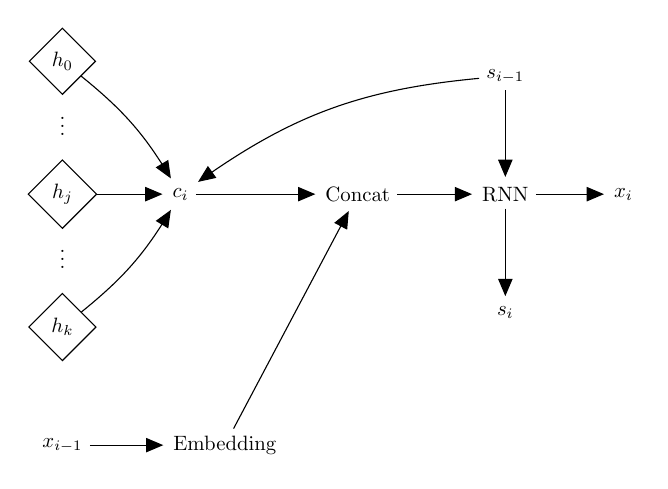
\begin{tikzpicture}[shorten >=1pt,node distance=1.5cm,on grid,auto, every node/.style={scale=0.75}]
        \node[] (x) {$x_{i-1}$};

        \node[draw,diamond] (h0) [above=of x] {$h_k$};
        \node[] (h1) [above=of h0, yshift=-0.75cm] {$\vdots$};
        \node[draw,diamond] (h2) [above=of h1, yshift=-1cm] {$h_j$};
        \node[] (h3) [above=of h2, yshift=-0.75cm] {$\vdots$};
        \node[draw,diamond] (h4) [above=of h3, yshift=-1cm] {$h_0$};

        \node[] (c) [right=of h2] {$c_i$};

        \node[]  (emb) [right=of x, xshift=0.75cm] {Embedding};
        \node[]  (concat) [right=of c, xshift=1cm] {Concat};
        \node[] (rnn) [right=of concat, xshift=0.5cm] {RNN};

        \node[] (xn) [right=of rnn] {$x_{i}$};

        \node[] (s) [above=of rnn] {$s_{i-1}$};


        \node[] (sn) [below=of rnn] {$s_i$};

        \path [->]
          (x) edge [] node {} (emb)
          (emb) edge [] node {} (concat)
          (c) edge [] node {} (concat)

          (h0) edge [bend right=10] node {} (c)
          (h2) edge [] node {} (c)
          (h4) edge [bend left=10] node {} (c)

          (concat) edge [] node {} (rnn)
          (s) edge [] node {} (rnn)
          (rnn) edge [] node {} (sn)
          (rnn) edge [] node {} (xn)
          (s) edge [bend right=15] node {} (c);

      \end{tikzpicture}
    \end{figure}
\end{frame}

%%%%%%%%%%%%%%%%%%%%%%%%%%%%%%%%%%%%%%%%%%%%%%%%%%%%%%%%%%%%%%%%%%%%%%%%%%%%%%%%
\section{(Simple) Attention Mechanisms}

\begin{frame}
\frametitle{Mean Attention}
\begin{equation*}
  \begin{split}
  \alpha_{ij} &= \frac{1}{S} \\
  c_i &= \frac{1}{S} \sum_j^S h_j = \sum_{j} \alpha_{ij} \cdot h_j
  \end{split}
\end{equation*}
\begin{itemize}
  \item Very simple and naive approach is to apply uniform weights to each encoding $h_j$
  \item Fancy way of saying average
  \item $S$ is the length of the source sentence
\end{itemize}
\end{frame}

\begin{frame}
\frametitle{Location Based: Laplace}
\begin{equation*}
  \begin{split}
  \alpha_{ij} &= f \left(j \mid i, b \right) = \frac{1}{2b} \exp \left( - \frac{\lvert j - i \rvert}{b} \right) \\
  c_i &= \sum_{j} \alpha_{ij} \cdot h_j
  \end{split}
\end{equation*}
\begin{itemize}
  \item Weighted by location in sequence
  \begin{itemize}
    \item Center a Laplace at $\mu=i$, scale $b$
    \item Weight is the probability of position $j$ relative to $i$
  \end{itemize}
  \item Penalizes elements away from the diagonal
  \item Heavier tail than a Gaussian
\end{itemize}
\end{frame}

\begin{frame}
\frametitle{Location Based: Gaussian}
\begin{equation*}
  \begin{split}
  \alpha_{ij} &= f \left(j \mid i, \sigma^2 \right) = \frac{1}{\sqrt{2\pi\sigma^2}} \exp \left( - \frac{\left( j - i \right)^2}{2\sigma^2} \right) \\
  c_i &= \sum_{j} \alpha_{ij} \cdot h_j
  \end{split}
\end{equation*}
\begin{itemize}
  \item Weighted by location in sequence
  \begin{itemize}
    \item Center a Gaussian at $\mu=i$, scale $\sigma$
    \item Weight is the probability of position $j$ relative to $i$
  \end{itemize}
  \item Smoother distribution closer to the diagonal
  \item Smaller tail than Laplace, so outliers are penalized more
\end{itemize}
\end{frame}

\begin{frame}
  \frametitle{Review: Laplace and Gaussian}
  \begin{figure}
    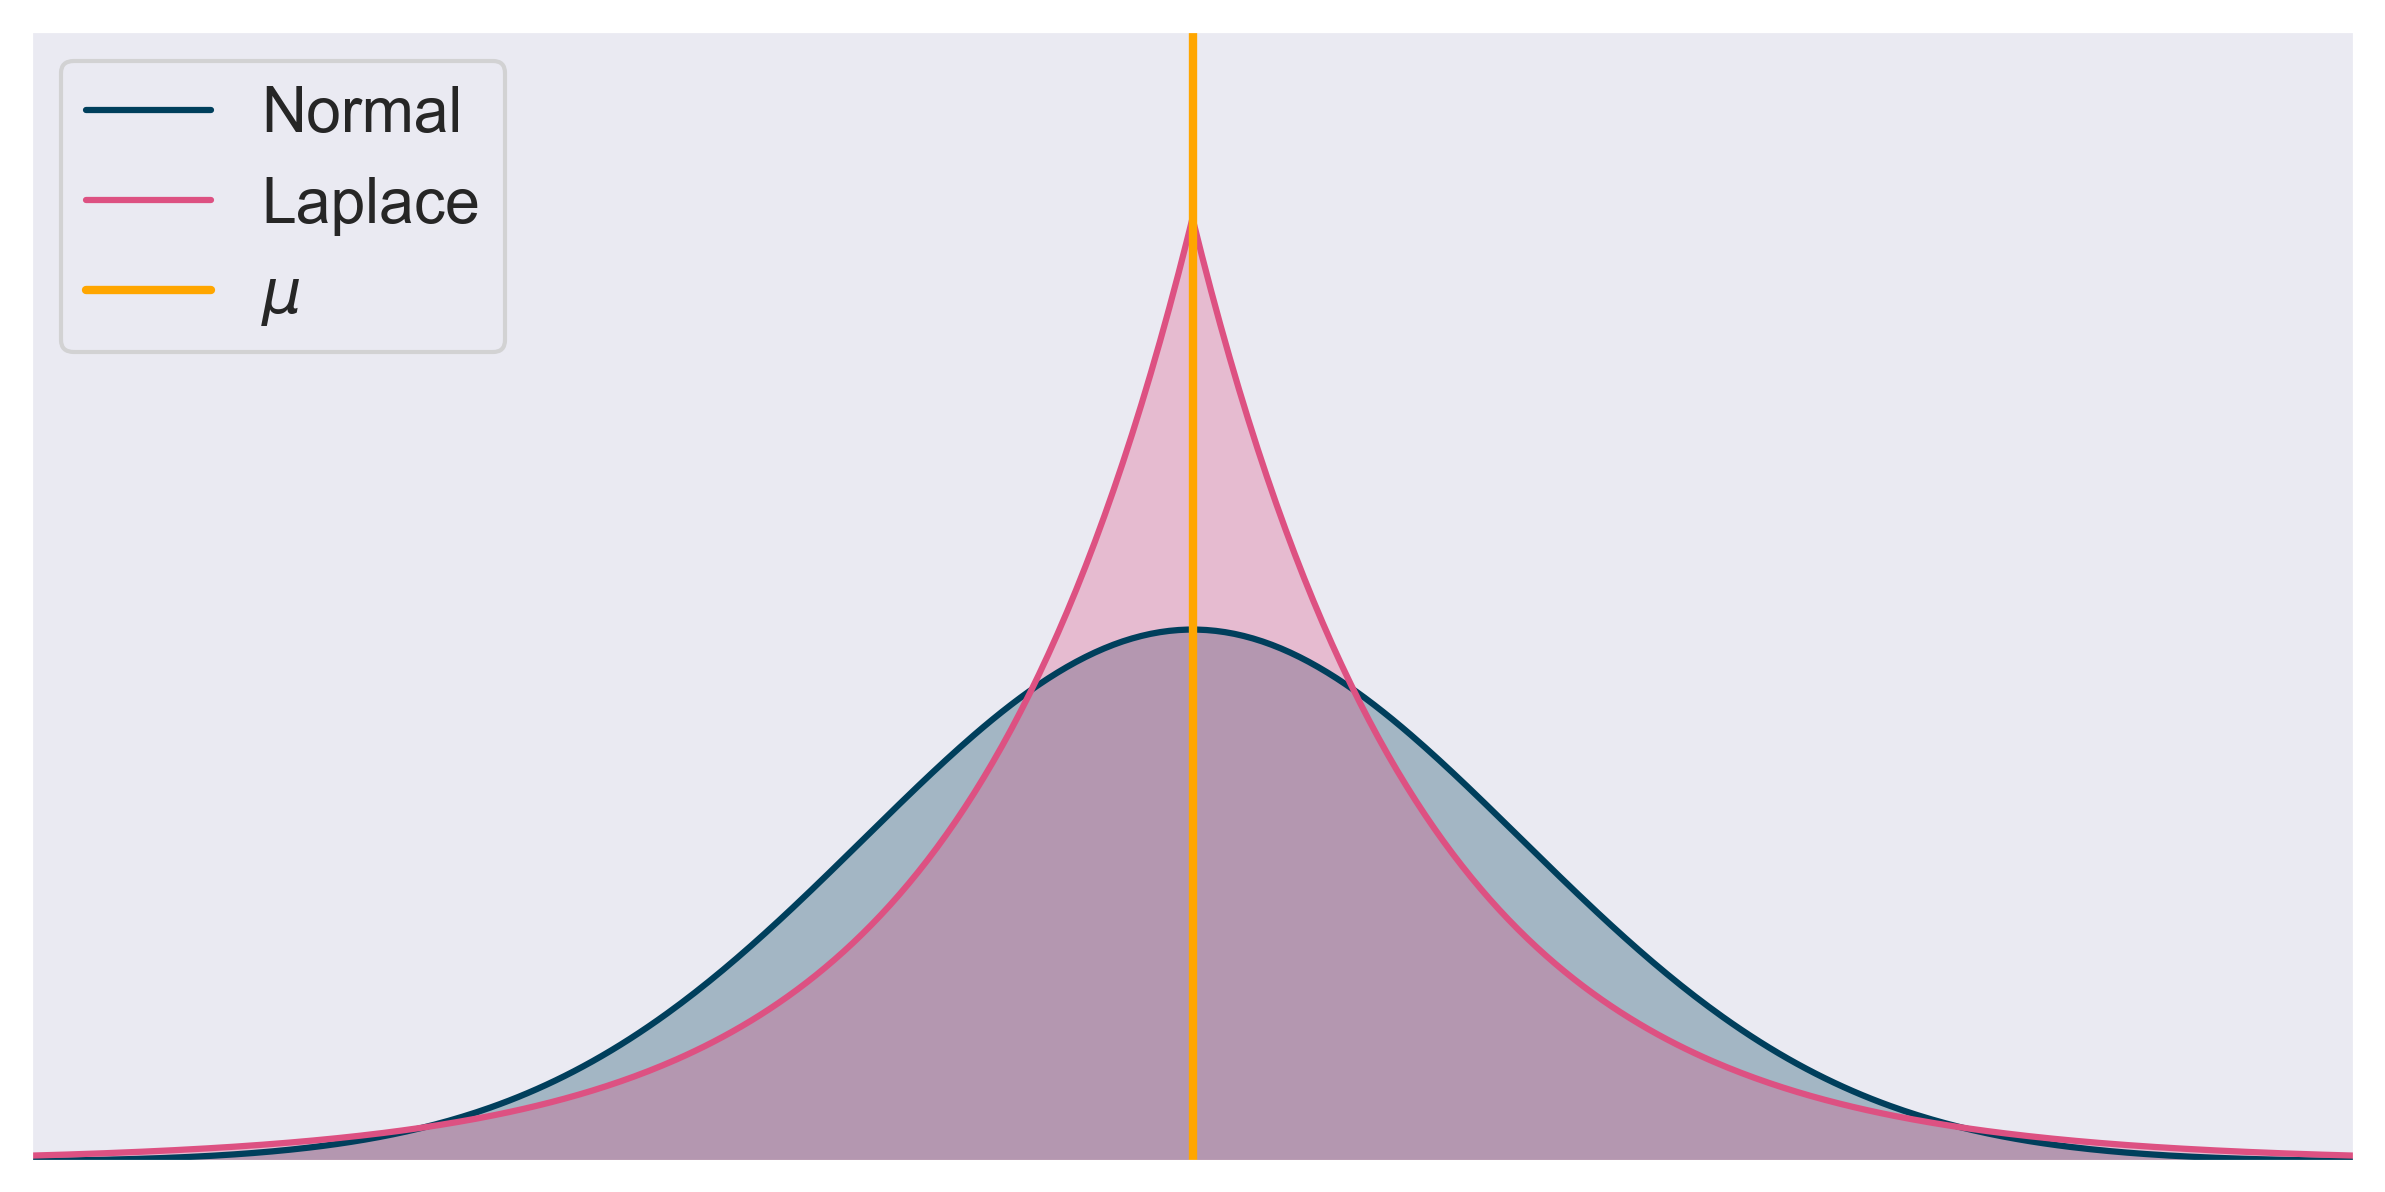
\includegraphics[width=\textwidth]{assets/dist}
  \end{figure}
\end{frame}

\begin{frame}
\frametitle{Visualizing Location-Based Distributions}
\begin{columns}
  \begin{column}{0.45\textwidth}
    \begin{figure}
      \centering
      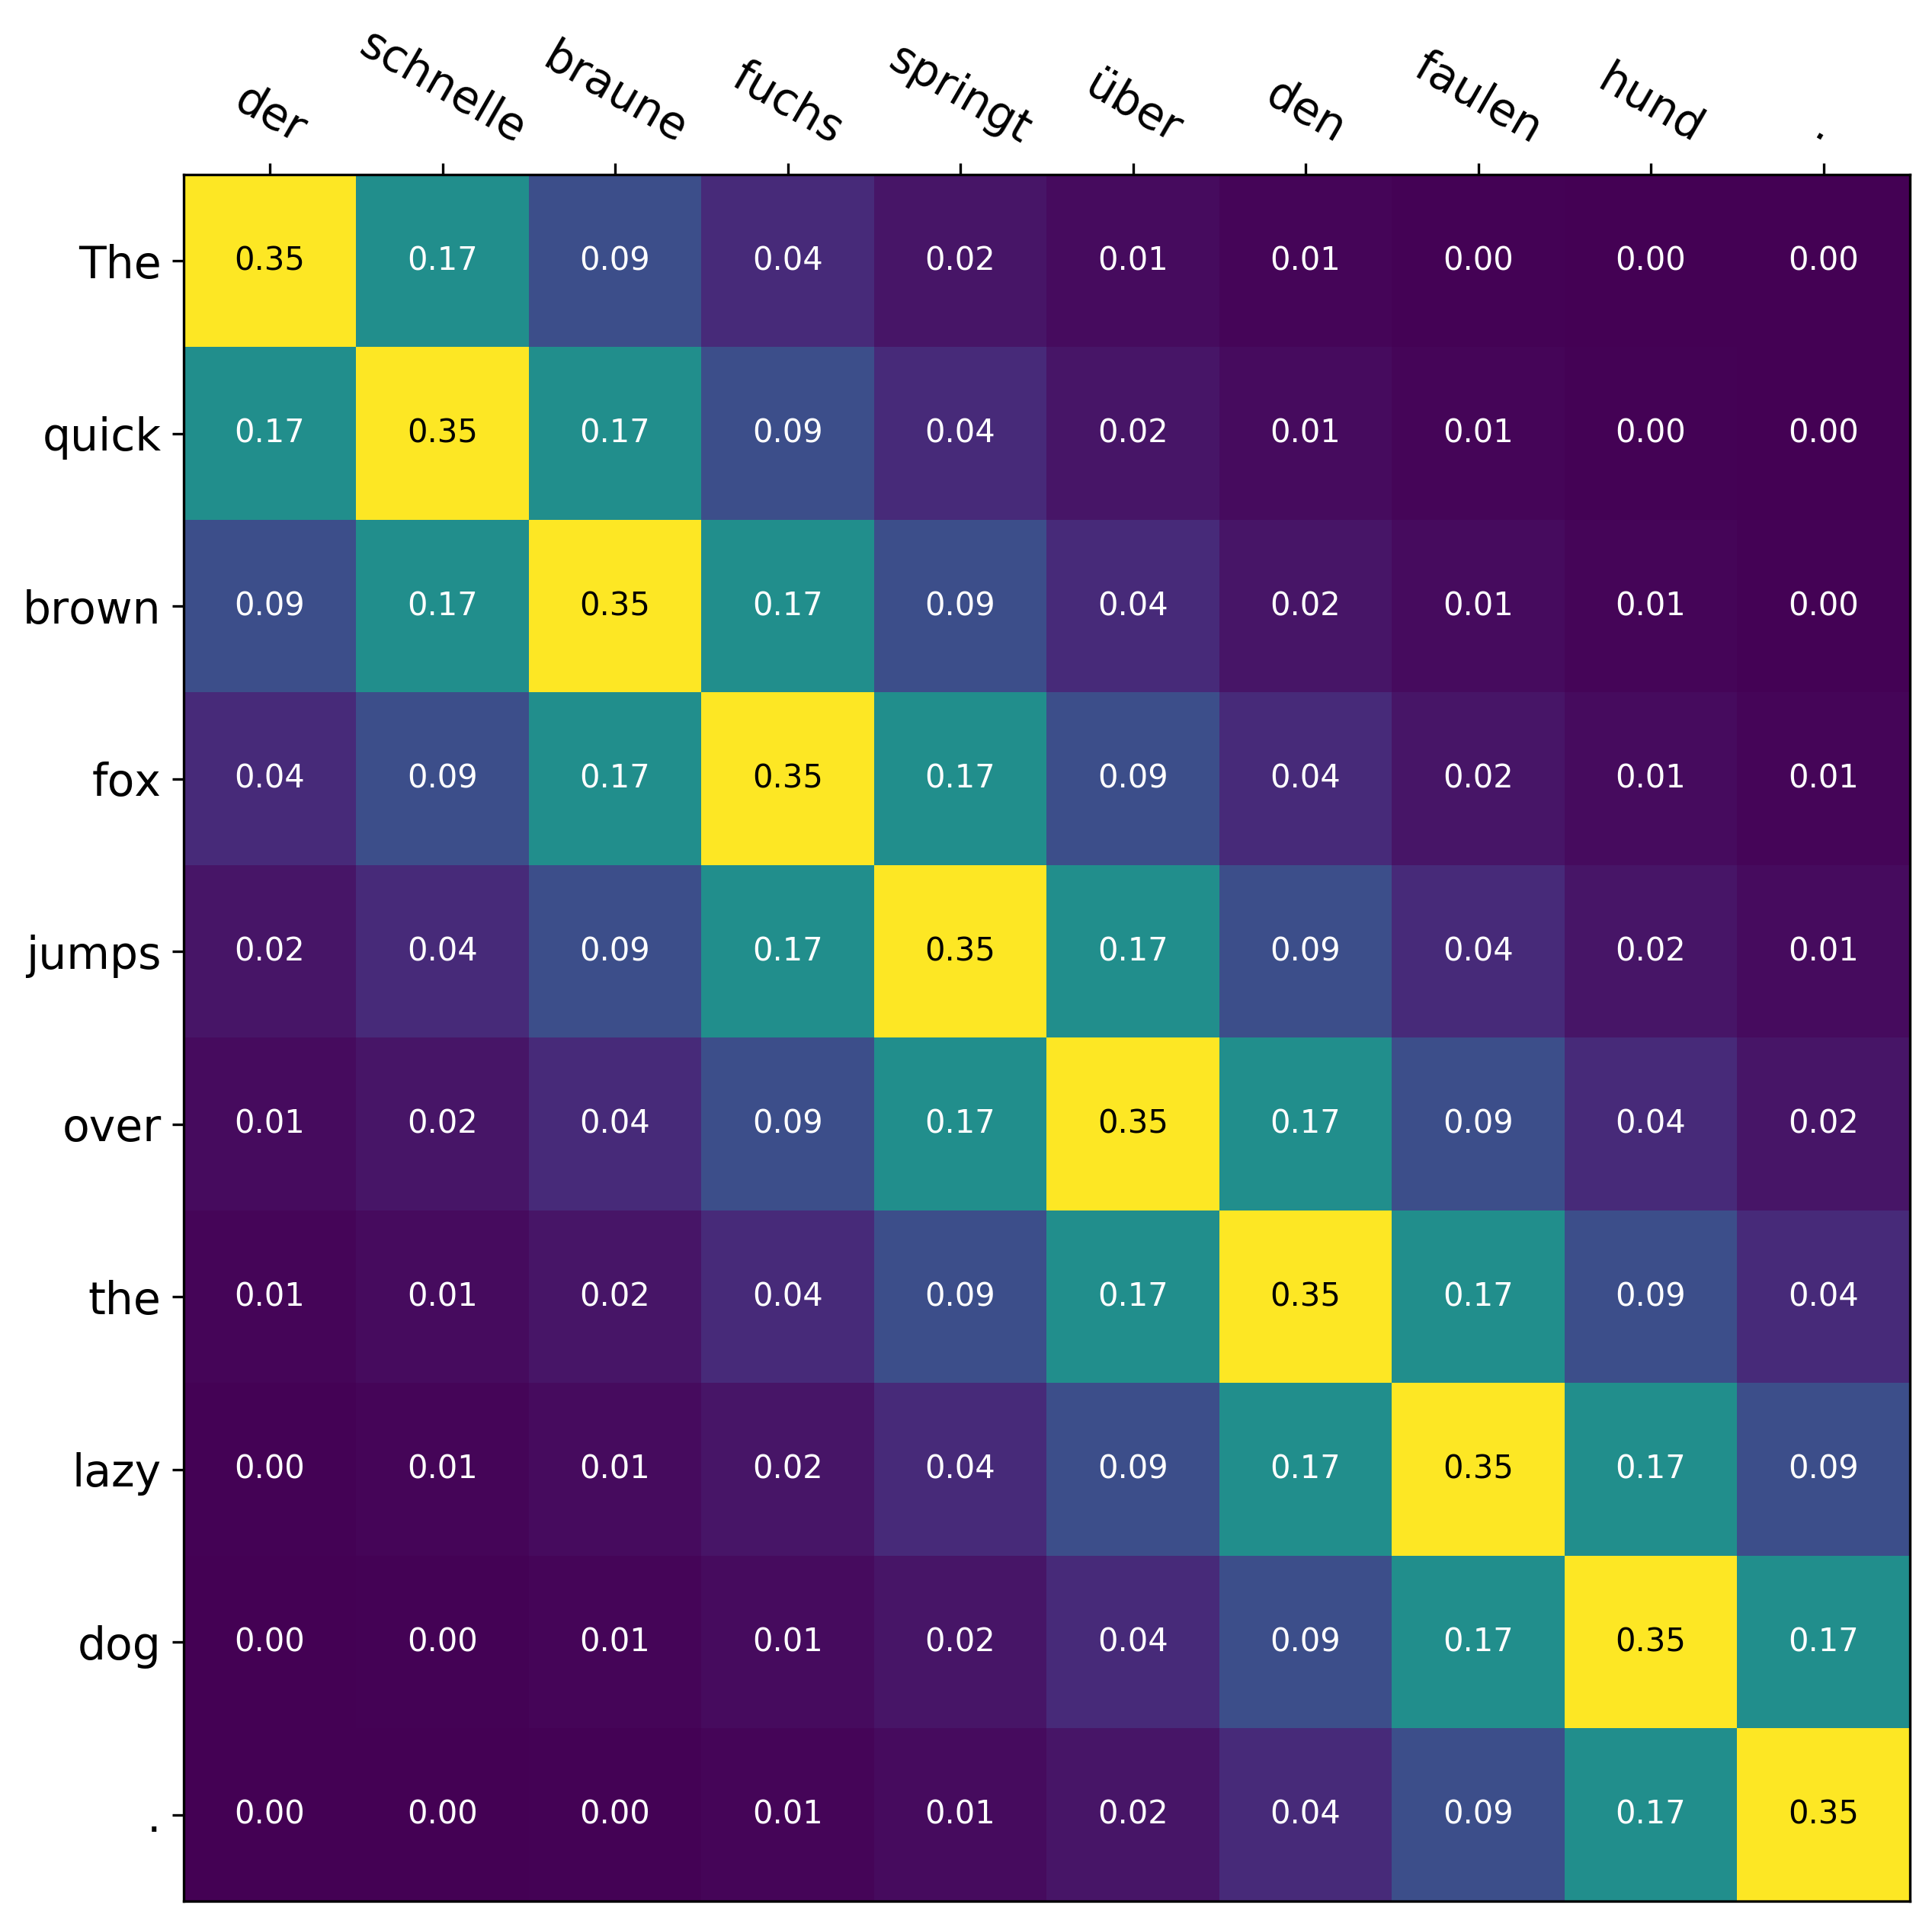
\includegraphics[width=4.75cm, valign=c]{assets/laplace}
      \caption{Laplace}
    \end{figure}
  \end{column}
  \begin{column}{0.45\textwidth}
    \begin{figure}
      \centering
      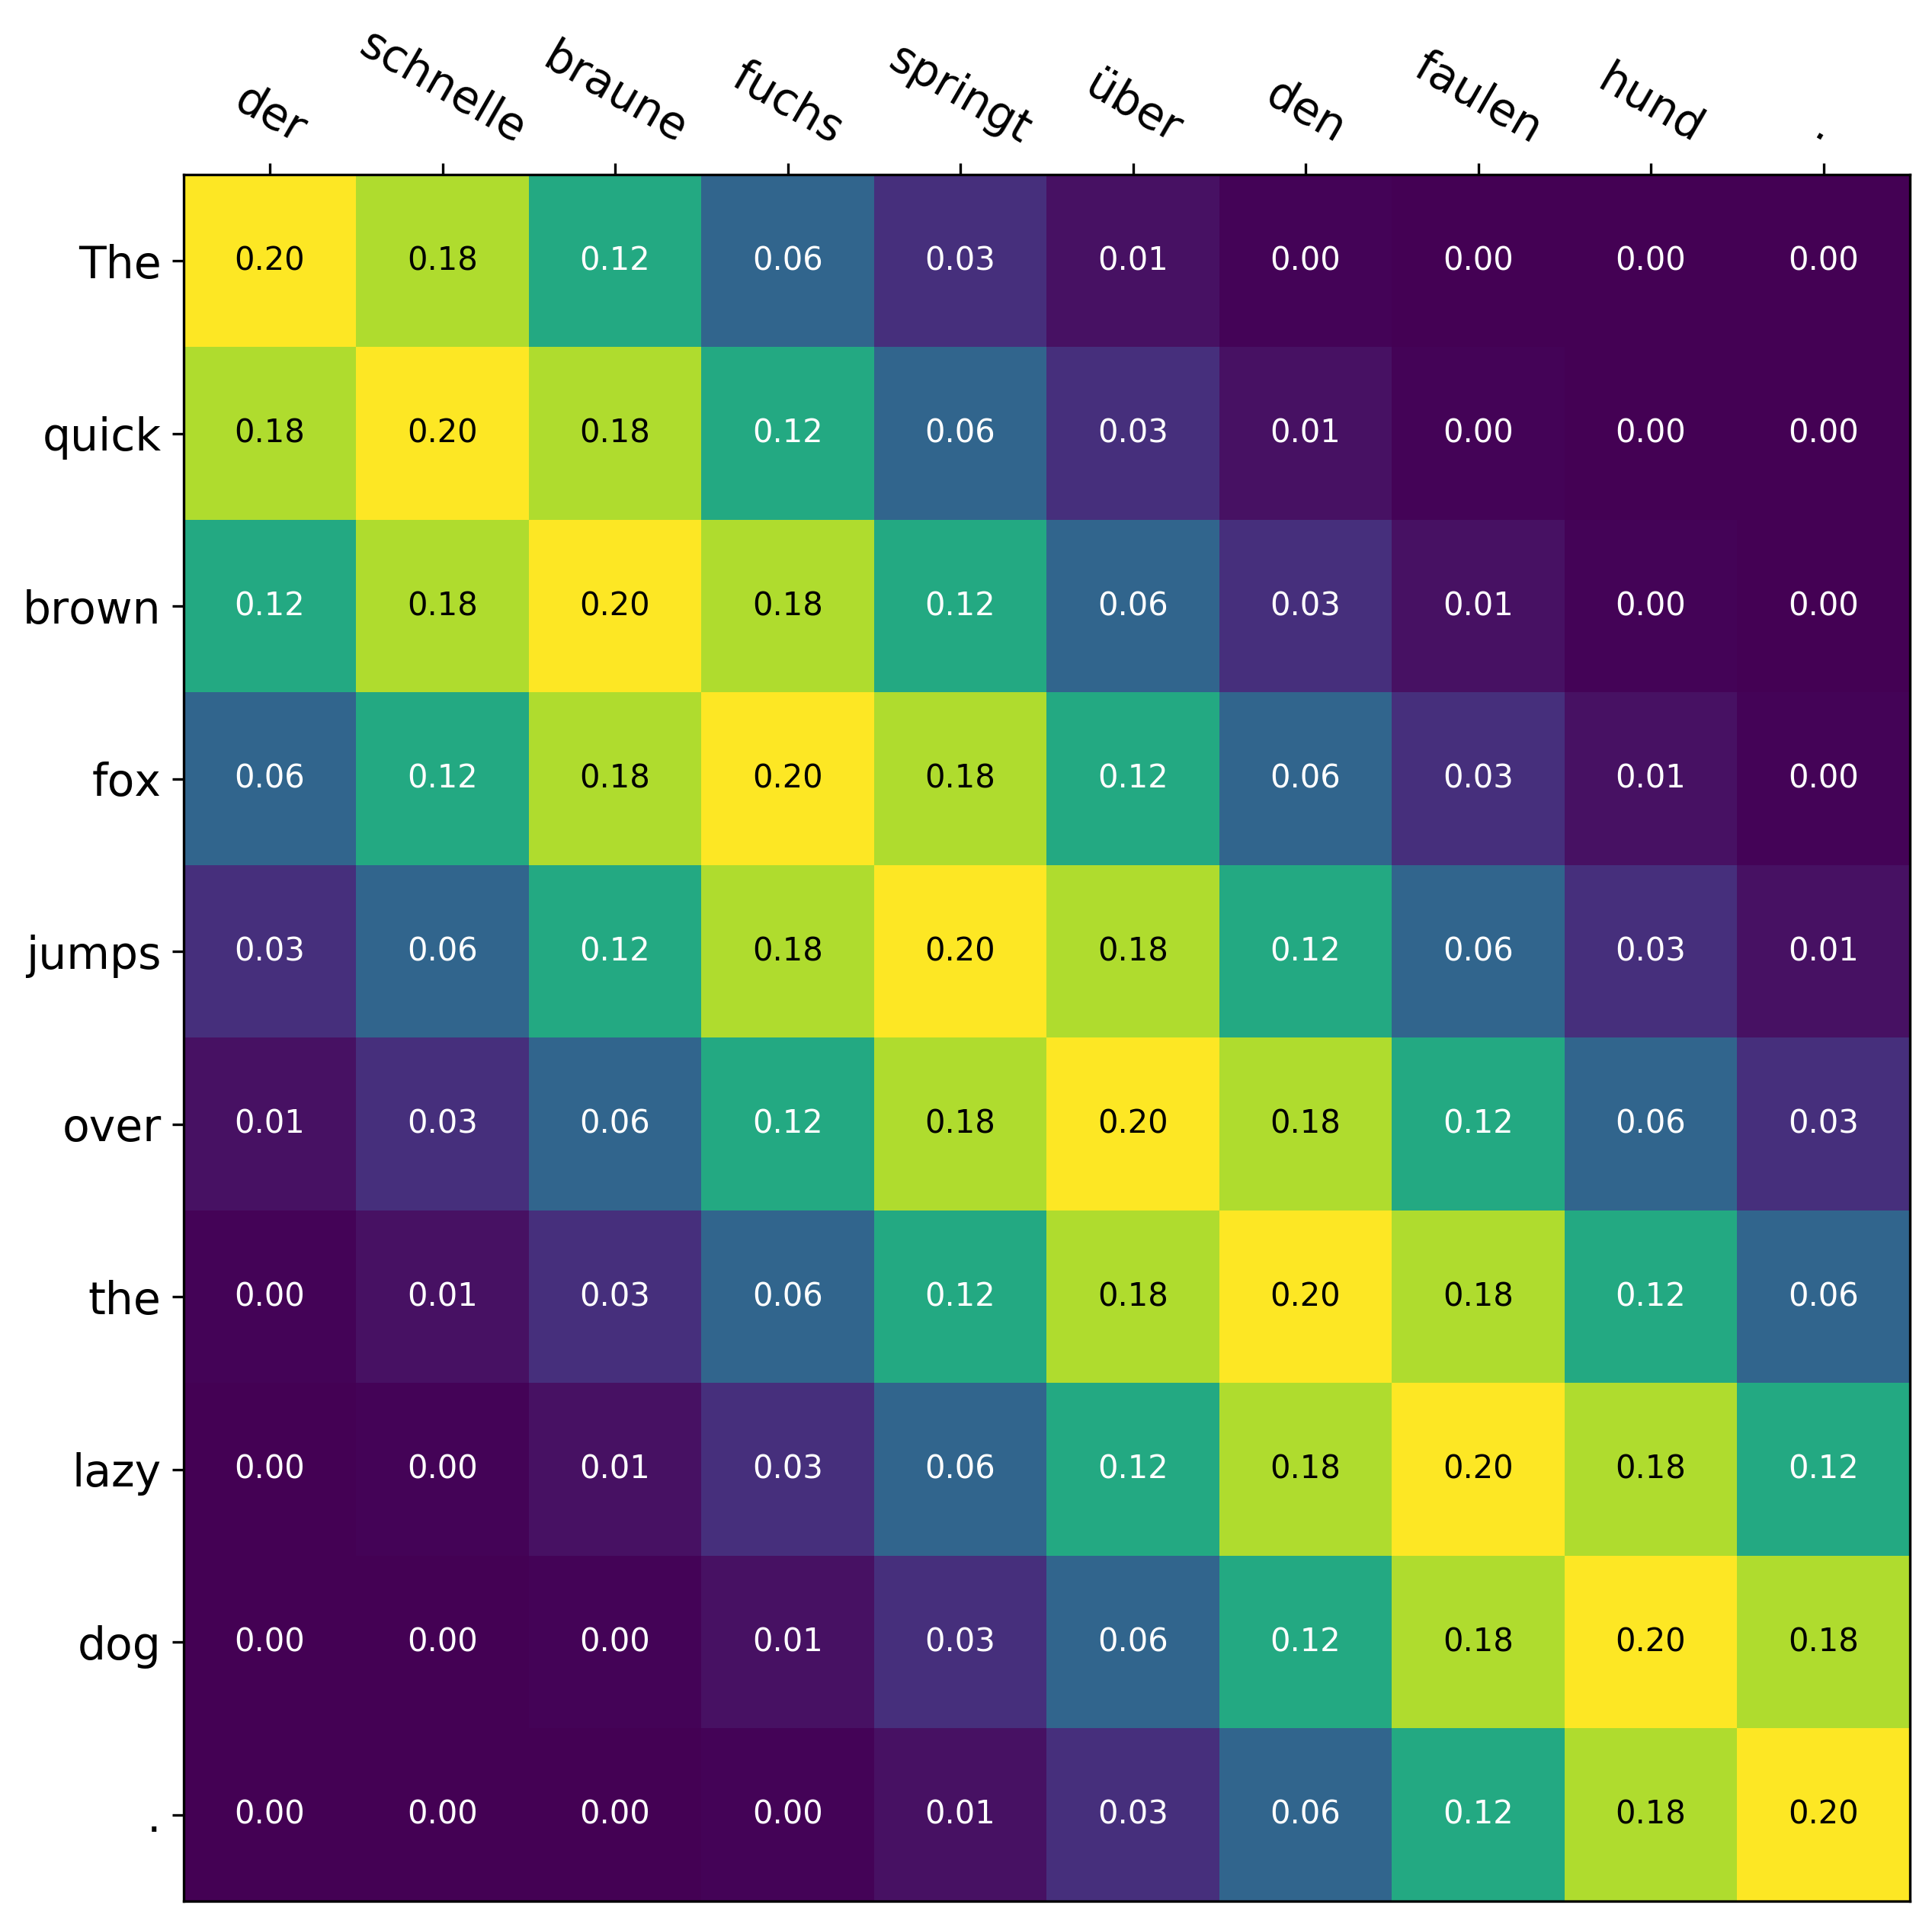
\includegraphics[width=4.75cm, valign=c]{assets/normal}
      \caption{Gaussian}
    \end{figure}
  \end{column}

\end{columns}
\end{frame}
%%%%%%%%%%%%%%%%%%%%%%%%%%%%%%%%%%%%%%%%%%%%%%%%%%%%%%%%%%%%%%%%%%%%%%%%%%%%%%%%
\section{(Parameter-based) Attention Mechanisms}

\begin{frame}
\frametitle{Parameter-based Attention}
% rework
\begin{itemize}
  \item Why not use learnable weights to effectively mix the encodings?
  \item Let deep learning figure out the alignment
  \item We now define a scoring function conditioned on the previous decoder state $s_{i-1}$ and input encodings $h_j$
\end{itemize}
\begin{equation*}
  a\left( s_{i-1}, h_j \right) = \;?
\end{equation*}
\begin{itemize}
  \item In order to constrain the weights to a valid distribution, we softmax
\end{itemize}
\begin{equation*}
  \begin{split}
    \alpha_{ij} &= \frac{\exp\left( a\left( s_{i-1}, h_j \right) \right)}{\sum_k \exp\left( a\left( s_{i-1}, h_k \right) \right)}\\
    c_i &= \sum_{j} \alpha_{ij} \cdot h_j
  \end{split}
\end{equation*}
\end{frame}



\begin{frame}
  \frametitle{Attention Computation Graph}
  \begin{figure}
      \centering
      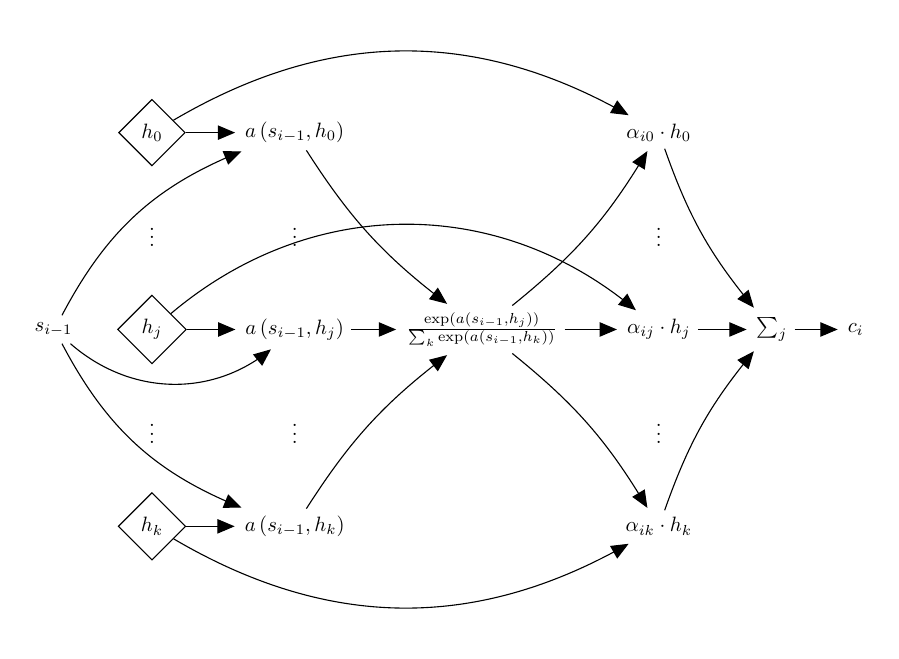
\begin{tikzpicture}[shorten >=1pt,node distance=1.25cm,on grid,auto, every node/.style={scale=0.75}]


        \node[draw,diamond]  (h2)  {$h_j$};
        \node[]  (h1) [above=of h2] {$\vdots$};
        \node[]  (h3) [below=of h2] {$\vdots$};
        \node[draw,diamond] [above=of h1]  (h0)  {$h_0$};
        \node[draw,diamond]  (h4) [below=of h3] {$h_{k}$};

        \node[] (s) [left=of h2] {$s_{i-1}$};

        \node[]   (a0) [right=of h0, xshift=0.75cm] {$a\left( s_{i-1}, h_0 \right)$};
        \node[]   (a1) [right=of h1, xshift=0.75cm] {$\vdots$};
        \node[]   (a2) [right=of h2, xshift=0.75cm] {$a\left( s_{i-1}, h_j \right)$};
        \node[]   (a3) [right=of h3, xshift=0.75cm] {$\vdots$};
        \node[]   (a4) [right=of h4, xshift=0.75cm] {$a\left( s_{i-1}, h_k \right)$};

        \node[] (softmax) [right=of a2, xshift=1.5cm] {$\frac{\exp\left( a\left( s_{i-1}, h_j \right) \right)}{\sum_k \exp\left( a\left( s_{i-1}, h_k \right) \right)}$};

        \node[] (mult0) [right=of a0, xshift=4.5cm] {$\alpha_{i0} \cdot h_0$};
        \node[] (mult1) [right=of a1, xshift=4.5cm] {$\vdots$};
        \node[] (mult2) [right=of a2, xshift=4.5cm] {$\alpha_{ij} \cdot h_j$};
        \node[] (mult3) [right=of a3, xshift=4.5cm] {$\vdots$};
        \node[] (mult4) [right=of a4, xshift=4.5cm] {$\alpha_{ik} \cdot h_k$};

        \node[] (sum) [right=of mult2, xshift=0.25cm] {$\sum_j$};

        \node[] (c) [right=of sum, xshift=-0.25cm] {$c_i$};

        \path [->]
          (h0) edge [] node[] {} (a0)
          (h2) edge [] node[] {} (a2)
          (h4) edge [] node[] {} (a4)

          (a0) edge [bend right=10] node[] {} (softmax)
          (a2) edge [] node[] {} (softmax)
          (a4) edge [bend left=10] node[] {} (softmax)

          (softmax) edge [bend right=10] node[] {} (mult0)
          (softmax) edge [] node[] {} (mult2)
          (softmax) edge [bend left=10] node[] {} (mult4)

          (mult0) edge [bend right=10] node[] {} (sum)
          (mult2) edge [] node[] {} (sum)
          (mult4) edge [bend left=10] node[] {} (sum)

          (sum) edge [] node[] {} (c)

          (h0) edge [bend left=30] node {} (mult0)
          (h2) edge [bend left=40] node {} (mult2)
          (h4) edge [bend right=30] node {} (mult4)

          (s) edge [bend left=20] node {} (a0)
          (s) edge [bend right=40] node {} (a2)
          (s) edge [bend right=20] node {} (a4);

      \end{tikzpicture}
    \end{figure}
\end{frame}

\begin{frame}
\frametitle{Bahdanau Attention}
\begin{equation*}
  a\left( s_{i-1}, h_j \right) = v_a^T \tanh \left( W_a s_{i-1} + U_a h_j + b \right)
\end{equation*}
\begin{itemize}
  \item $W_a$, $U_a$, are learnable matrices
  \item $v_a$, $b$ are learnable vectors
  \item Output is a scalar value
  \item AKA: Additive Attention, Concat Attention
\end{itemize}
\end{frame}

\begin{frame}
  \frametitle{Bahdanau Attention Visual}
  \begin{figure}
    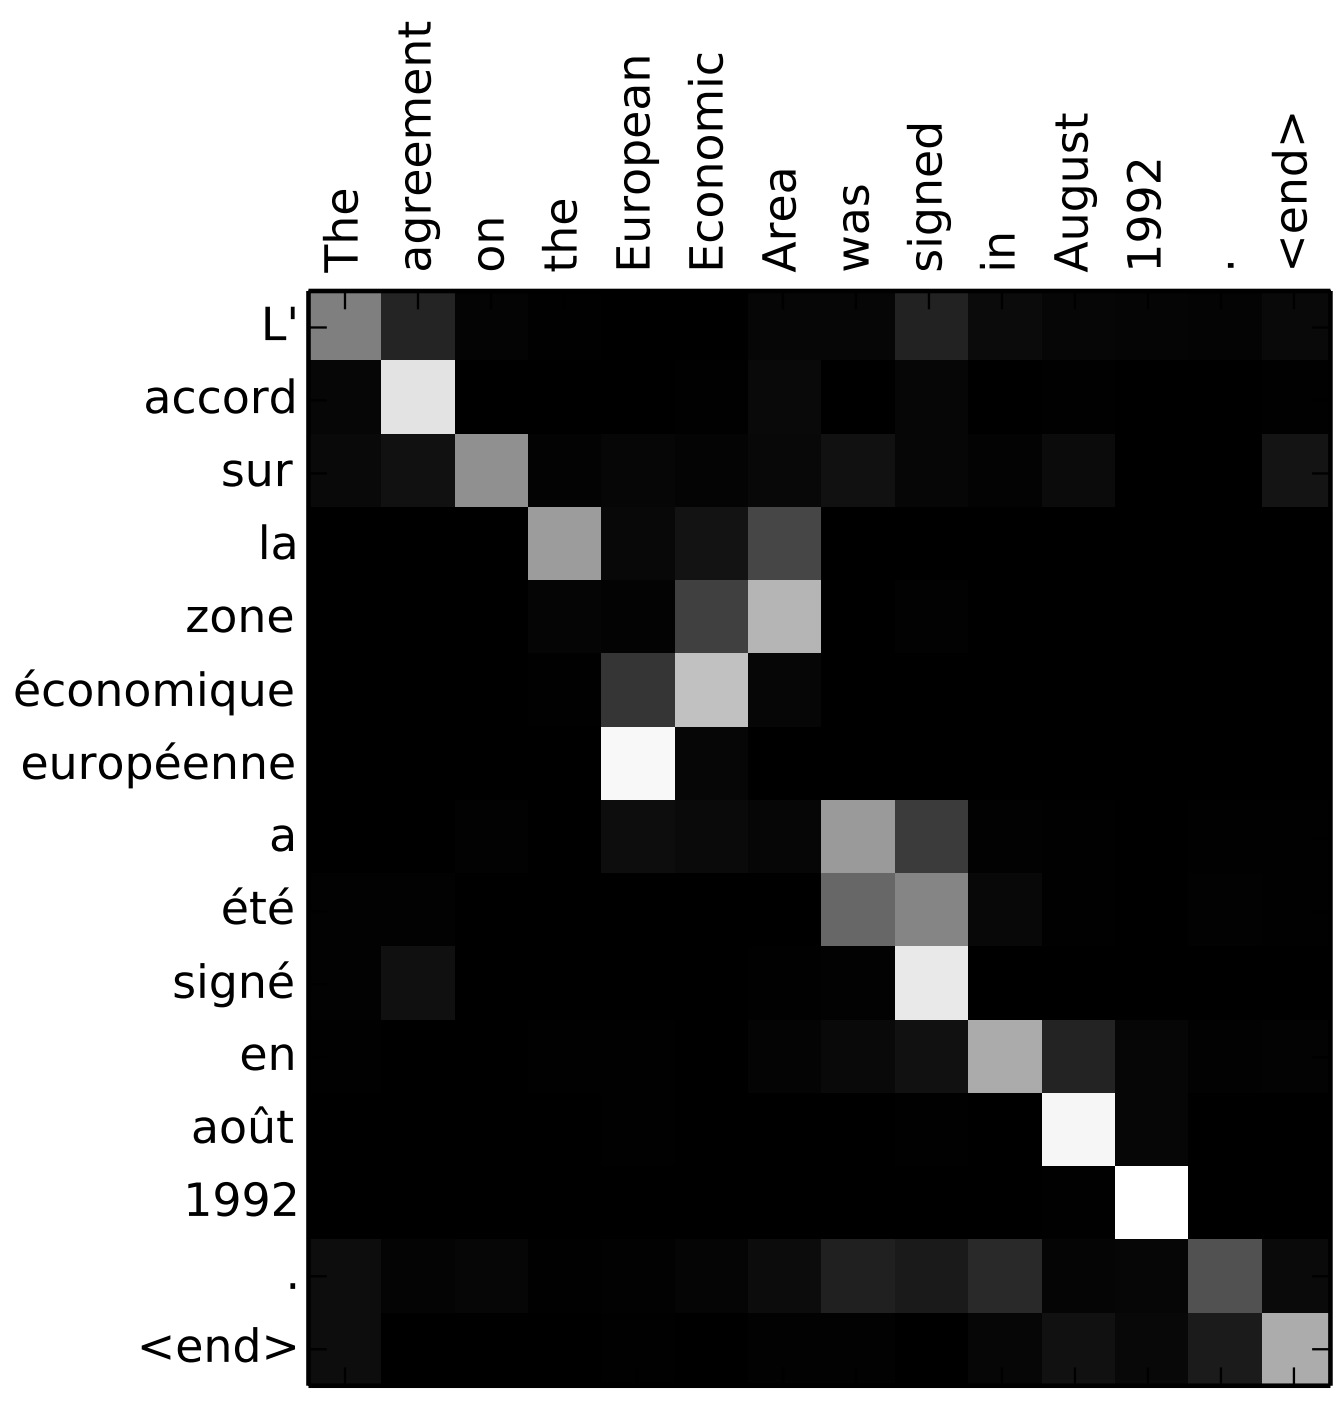
\includegraphics[height=7.25cm]{assets/concat1}
  \end{figure}
\end{frame}

\begin{frame}
  \frametitle{Bahdanau Attention Visual}
  \begin{figure}
    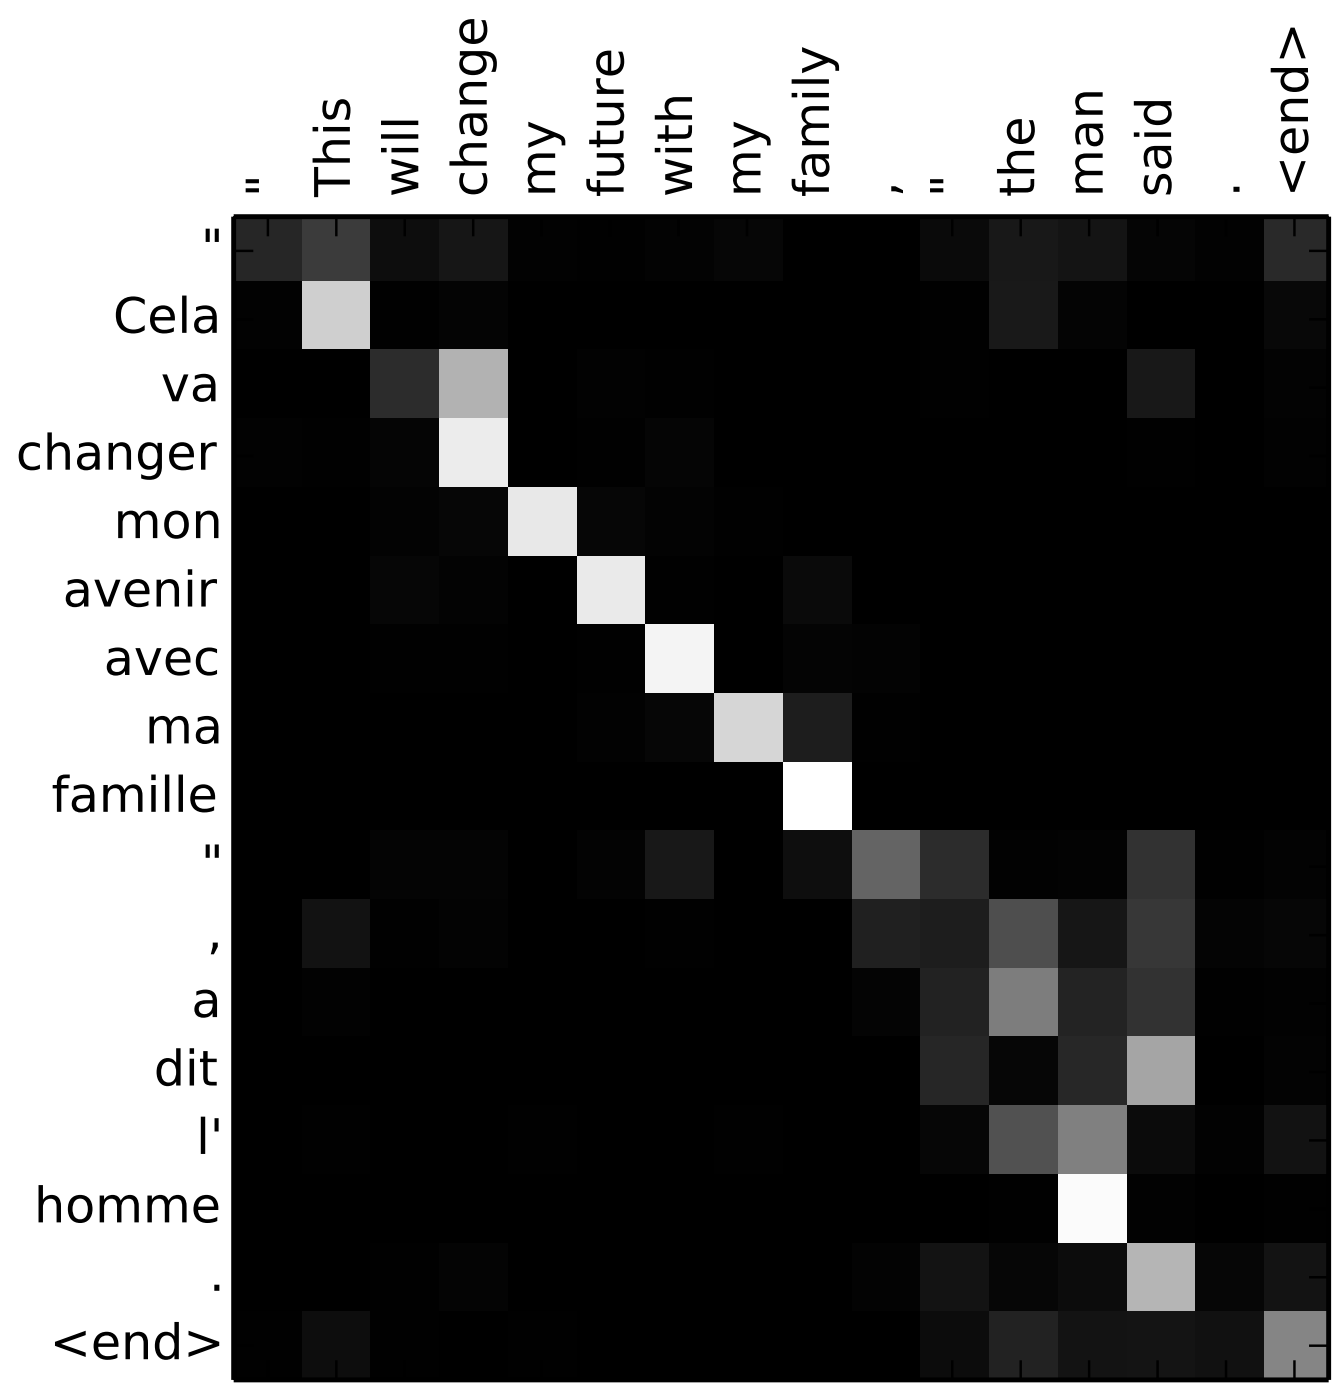
\includegraphics[height=7.25cm]{assets/concat2}
  \end{figure}
\end{frame}


\begin{frame}
\frametitle{Luong Attention: Dot Product}
\begin{equation*}
  a\left( s_{i-1}, h_j \right) = s_{i-1}^T h_j
\end{equation*}
\begin{itemize}
  \item Notice: No Learnable Parameters
  \item Simple dot product between decoder state and encoding
  \item Output is a scalar value
\end{itemize}
\end{frame}

\begin{frame}
\frametitle{Luong Attention: Scaled Dot Product}
\begin{equation*}
  a\left( s_{i-1}, h_j \right) = \frac{1}{\sqrt{\lvert h_j \rvert}} s_{i-1}^T h_j
\end{equation*}
\begin{itemize}
  \item Rescale the dot product accoridng to the dimensionality of the vectors
  \item \textbf{Why?} Because for large dimensionality, the dot-product is large in magnitude, resulting in small gradients from the softmax
  \item Output is a scalar value
\end{itemize}
\end{frame}

\begin{frame}
\frametitle{Luong Attention: General}
\begin{equation*}
  a\left( s_{i-1}, h_j \right) = s_{i-1}^T W_a h_j
\end{equation*}
\begin{itemize}
  \item Allow a learnable matrix $W_a$ inbetween the states
  \item AKA a Bilinear Layer: $x_0^T A x_1$
  \item Output is a scalar value
\end{itemize}
\end{frame}

\begin{frame}
\frametitle{Luong Attention: Location Attention}
\begin{equation*}
  a\left( s_{i-1}, h_j \right) = W_a s_{i-1}
\end{equation*}
\begin{itemize}
  \item An approach to reweight exclusively on the decoder state
  \item Single learnable matrix $W_a$
  \item Output is vector of fixed-length
  \item \textbf{Footnote:} For short sentences, only use the top part of the vector. For long sentences, ignore words near the end.
  \item \textbf{Note:} Implies that this only works for fixed-length sentences!
\end{itemize}
\end{frame}


\begin{frame}
  \frametitle{Luong Attention Visual}
  \begin{columns}
  \begin{column}{0.45\textwidth}
  \begin{figure}
    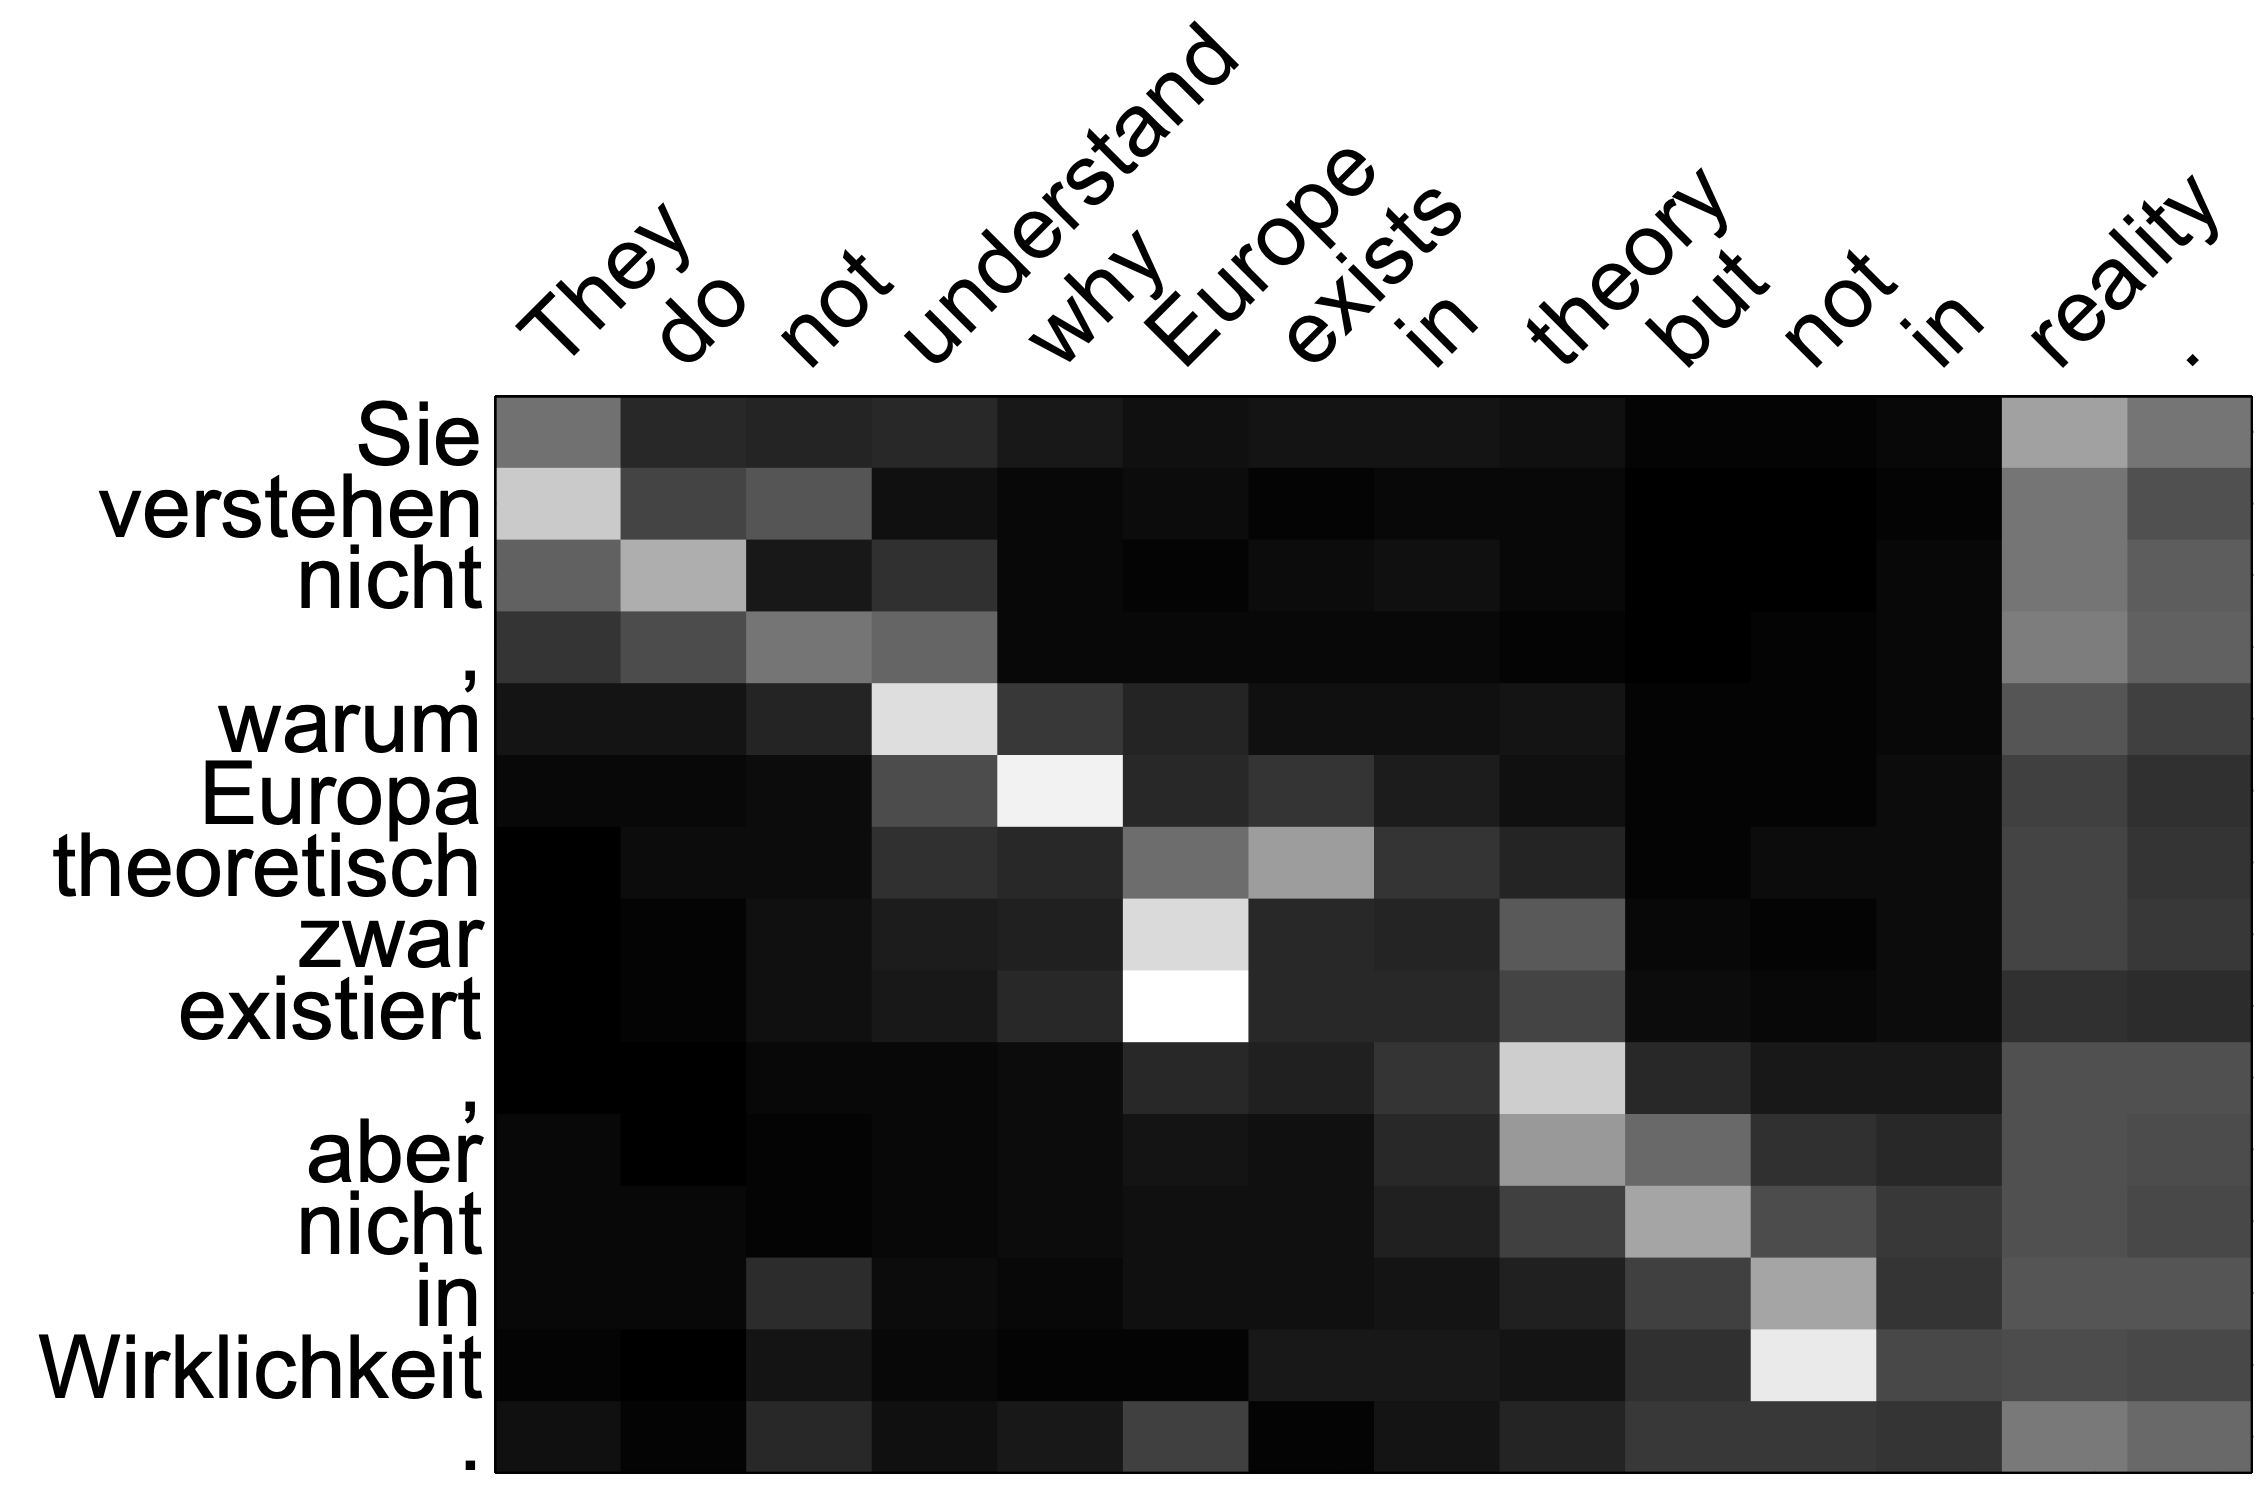
\includegraphics[width=5cm]{assets/global}
    \caption{Luong Attention}
  \end{figure}
\end{column}
\begin{column}{0.45\textwidth}
  \begin{figure}
    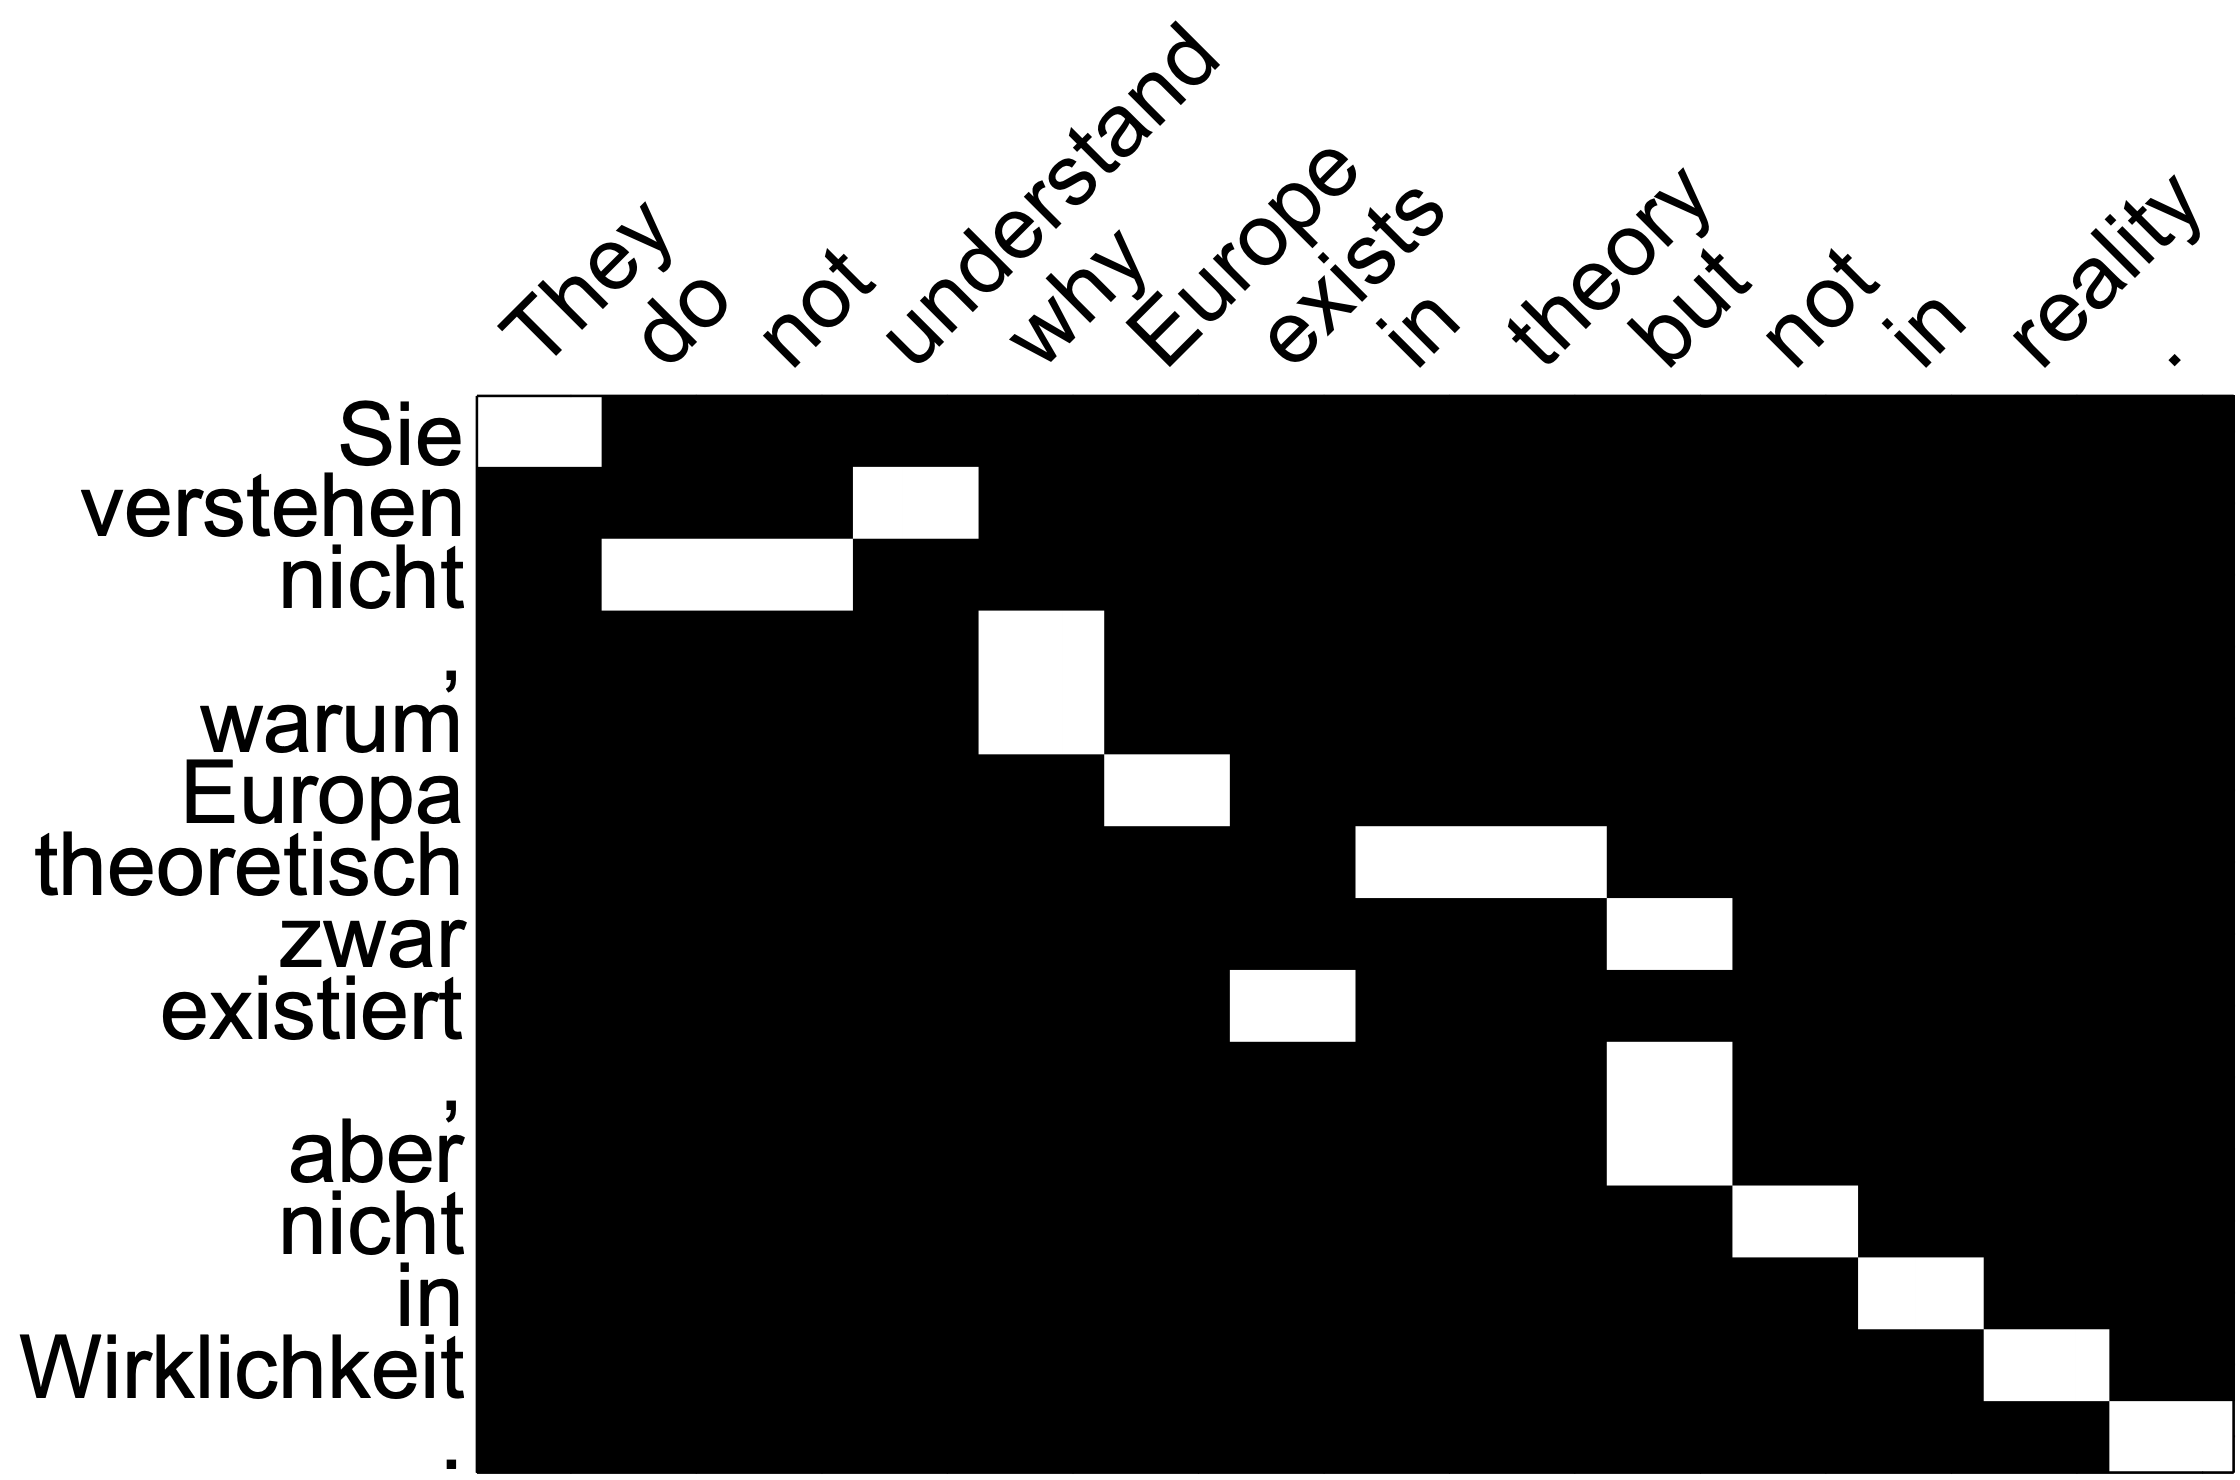
\includegraphics[width=5cm]{assets/gold}
    \caption{Gold Alignments}
  \end{figure}
\end{column}
  \end{columns}
\end{frame}

%%%%%%%%%%%%%%%%%%%%%%%%%%%%%%%%%%%%%%%%%%%%%%%%%%%%%%%%%%%%%%%%%%%%%%%%%%%%%%%%
\section{(Advanced) Attention Mechanisms}

\begin{frame}
  \frametitle{Luong Attention: Local Attention}
  \begin{itemize}
    \item What if we focused on a window instead of all the vectors?
    \item This approach is known as \textit{local} attention
    \item Before, we were using \textit{global} attention
  \end{itemize}
\end{frame}

\begin{frame}
  \frametitle{Luong Attention: Local Attention}
  \begin{itemize}
    \item Define a window $\mathcal{W}$ of size $2D$ at alignment point $p_t$:
  \end{itemize}
  \begin{equation*}
    \mathcal{W} = \left[ p_t - D, p_t + D \right]
  \end{equation*}
  \begin{itemize}
    \item Our context vector is now an average over this window
  \end{itemize}
  \begin{equation*}
    c_i = \sum_{j \in \mathcal{W}} \alpha_{ij} \cdot h_j
  \end{equation*}
\end{frame}

\begin{frame}
  \frametitle{Luong Attention: Local Attention}
  \begin{itemize}
    \item How do we select $p_t$, the alignment position?
    \item \textbf{Monotonic} alignment - set $p_t = t$
    \begin{itemize}
      \item Assumes \texttt{src} and \texttt{trg} are roughly monotonically aligned
    \end{itemize}
    \item \textbf{Predictive} alignment - predict the aligned position
  \end{itemize}
\end{frame}

\begin{frame}
  \frametitle{Luong Attention: Local Predictive Attention}
  \begin{equation*}
    p_t = S \cdot \sigma \left( v_p^T \tanh \left( W_p \cdot s_{i-1} \right) \right)
  \end{equation*}
  \begin{itemize}
    \item \textbf{Predictive} alignment allows for learnable positions
    \item $S$ is the length of the source sentence
    \item $W_p$ and $v_p$ are learnable
    \item Sigmoid enforces the constraint $p_t \in \left[ 0, S \right]$
  \end{itemize}
\end{frame}

\begin{frame}
  \frametitle{Luong Attention: Local Predictive Attention}
  \begin{equation*}
    a_{p} \left( s_{i-1}, h_j \right) = a\left( s_{i-1}, h_j \right) \cdot \exp \left( -\frac{ \left(j - p_t\right)^{2} }{2\sigma^2} \right)
  \end{equation*}
  \begin{itemize}
    \item Use a gaussian penalty to favor words near $p_t$
    \item Note: $p_t \in \mathbb{R}$, $j \in \mathbb{Z}$
    \item $j$ is the \textit{integer} position of the encoding within the window
    \item Empirically set $\sigma = \frac{D}{2}$
    \item $a\left( s_{i-1}, h_j \right)$ is any previous attention mechanism
  \end{itemize}
\end{frame}

\begin{frame}
  \frametitle{Luong Attention Visuals}
  \begin{columns}
    \begin{column}{0.45\textwidth}
      \vspace{-5mm}
    \begin{figure}
      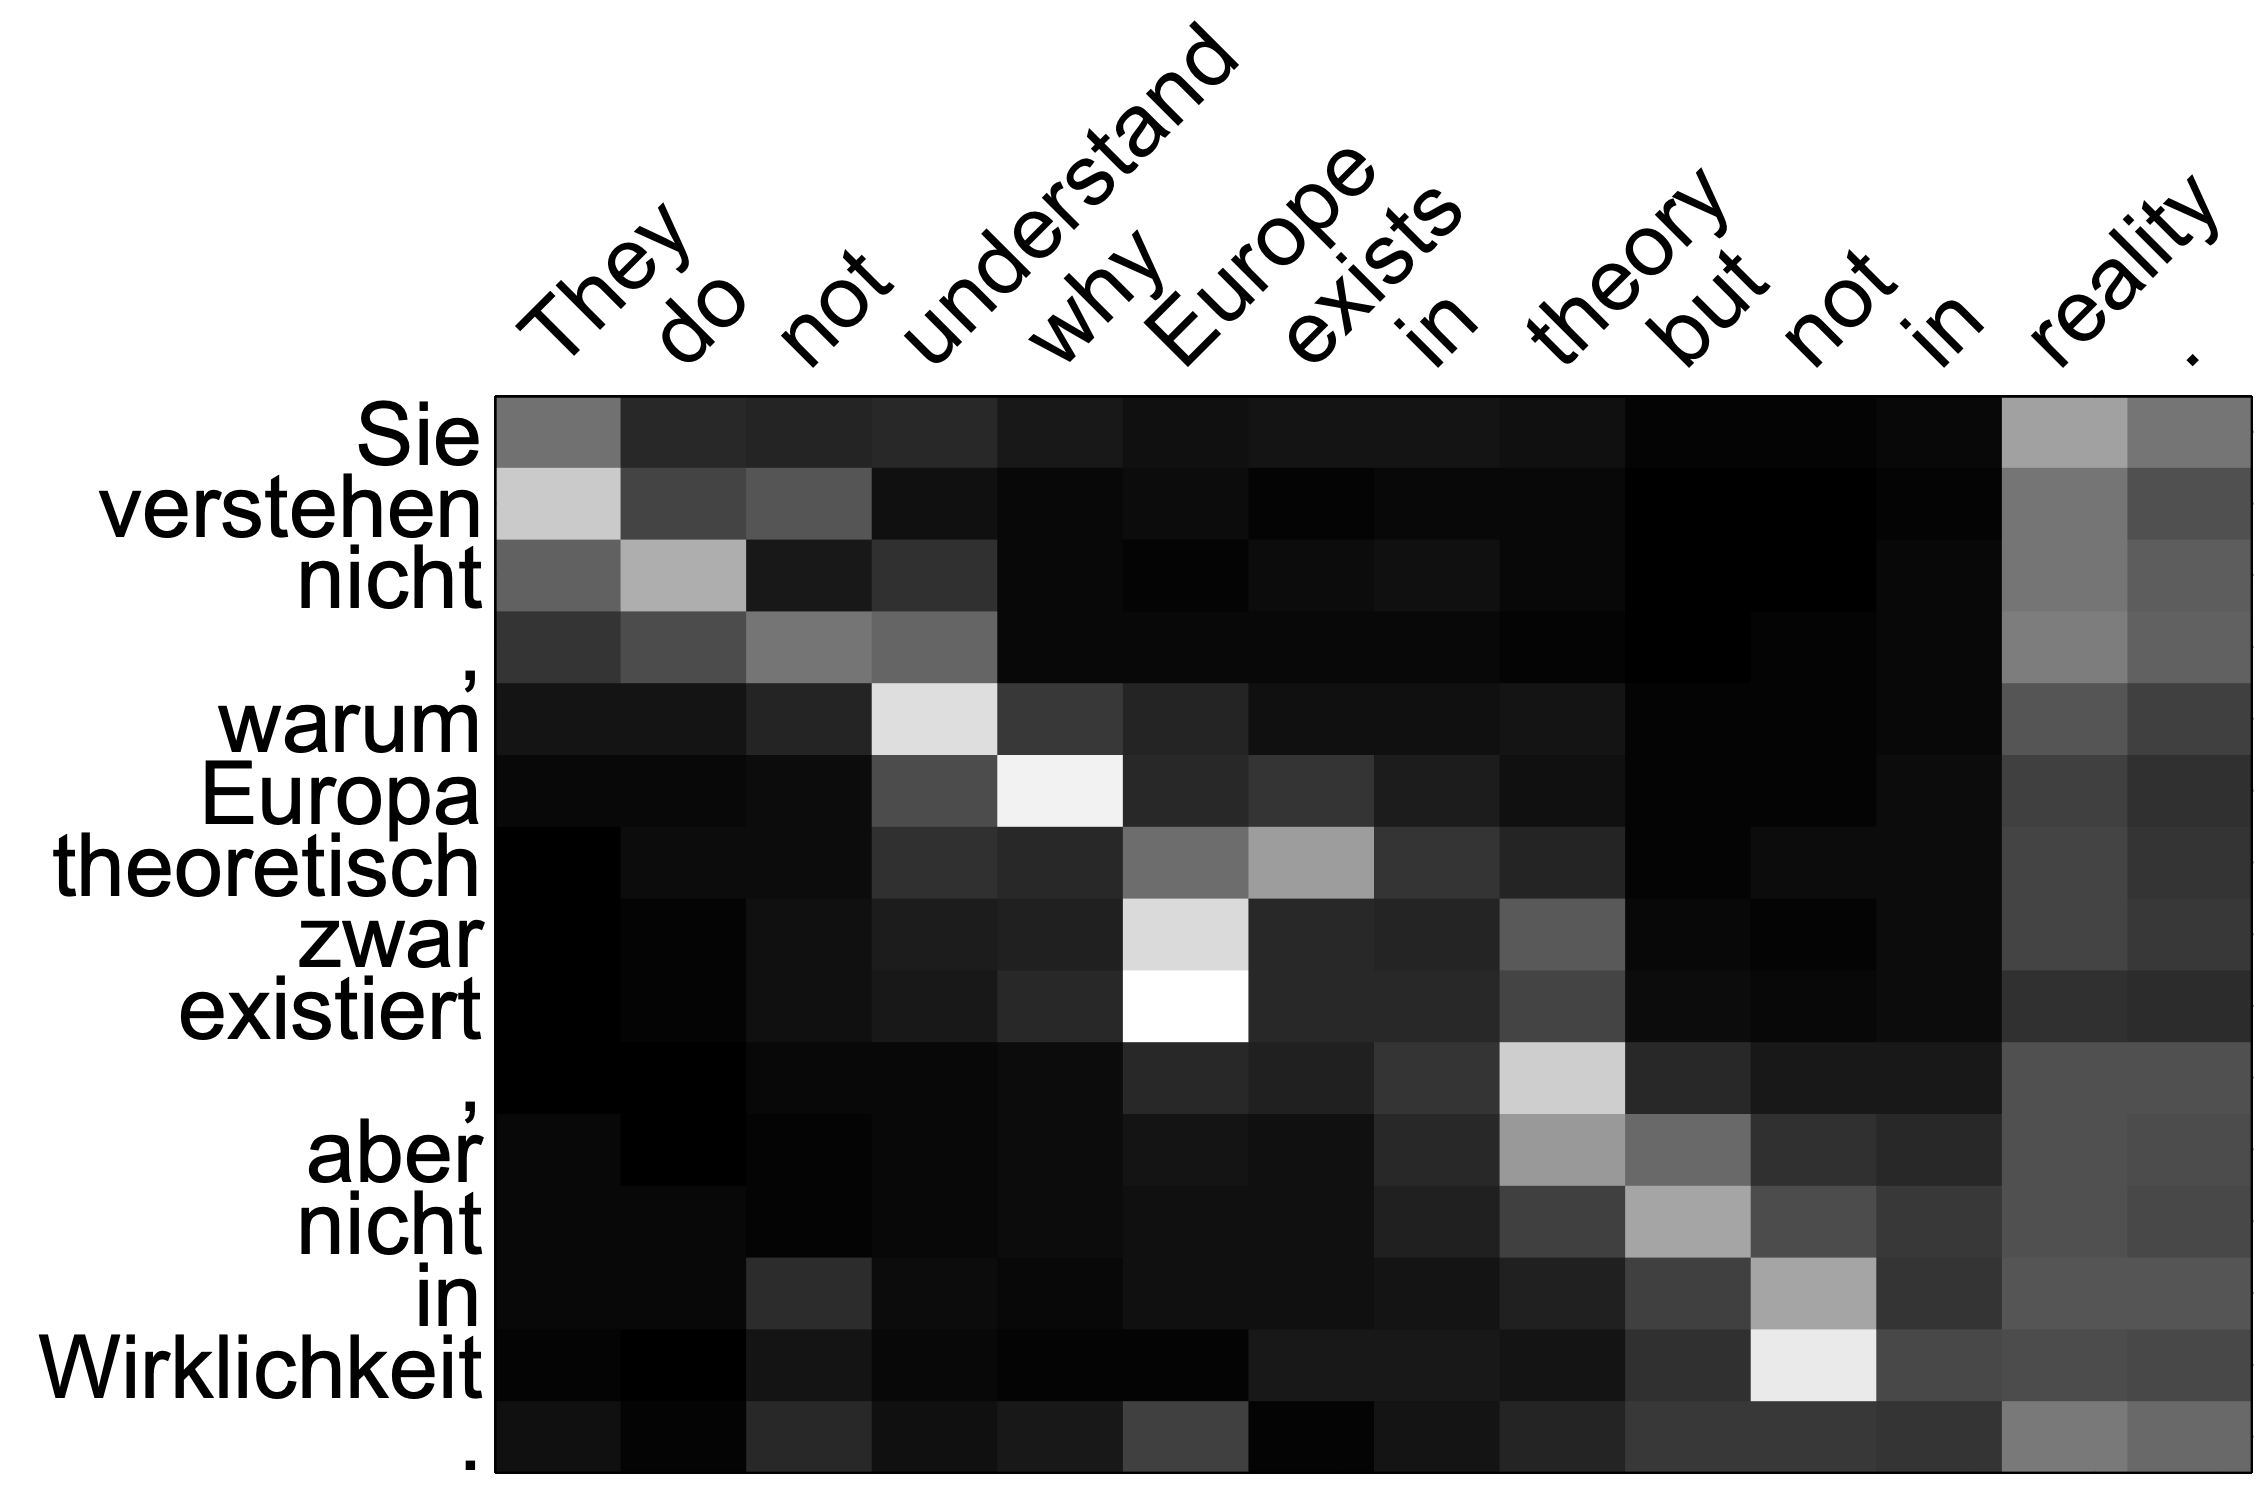
\includegraphics[width=0.95\textwidth]{assets/global}
      \caption{Global Attention}
    \end{figure}
    \vspace{-7mm}
    \begin{figure}
      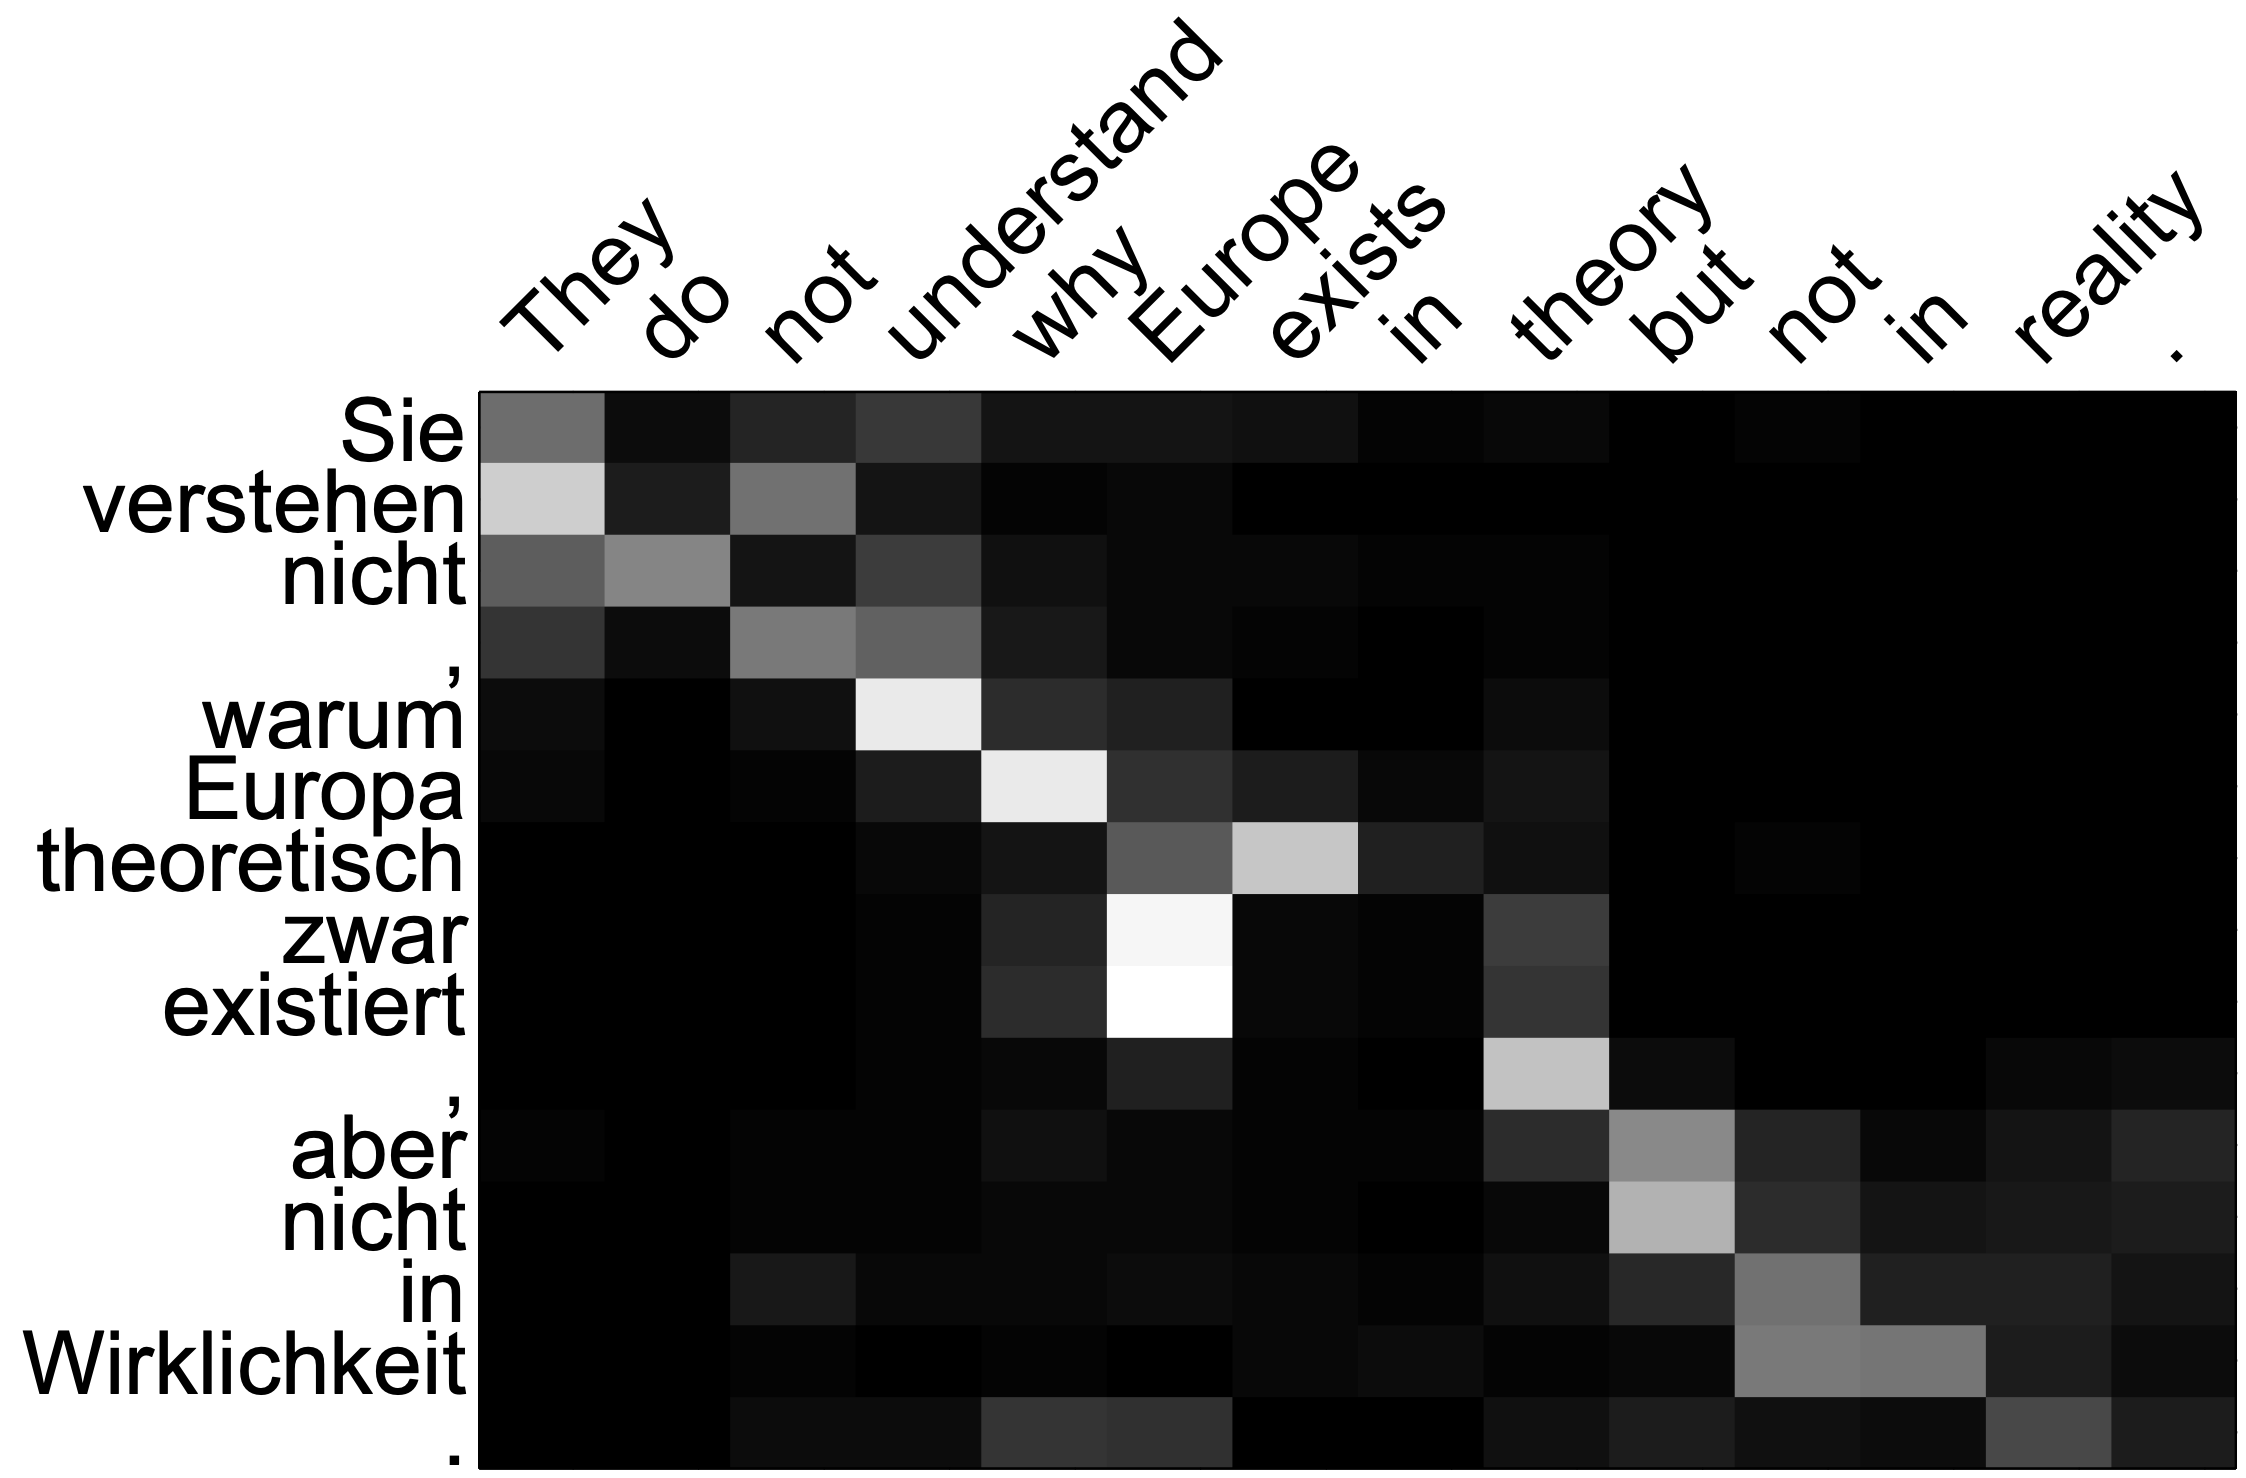
\includegraphics[width=0.95\textwidth]{assets/local_p}
      \caption{Local-P}
    \end{figure}
    \end{column}

    \begin{column}{0.45\textwidth}
      \vspace{-5mm}
    \begin{figure}
      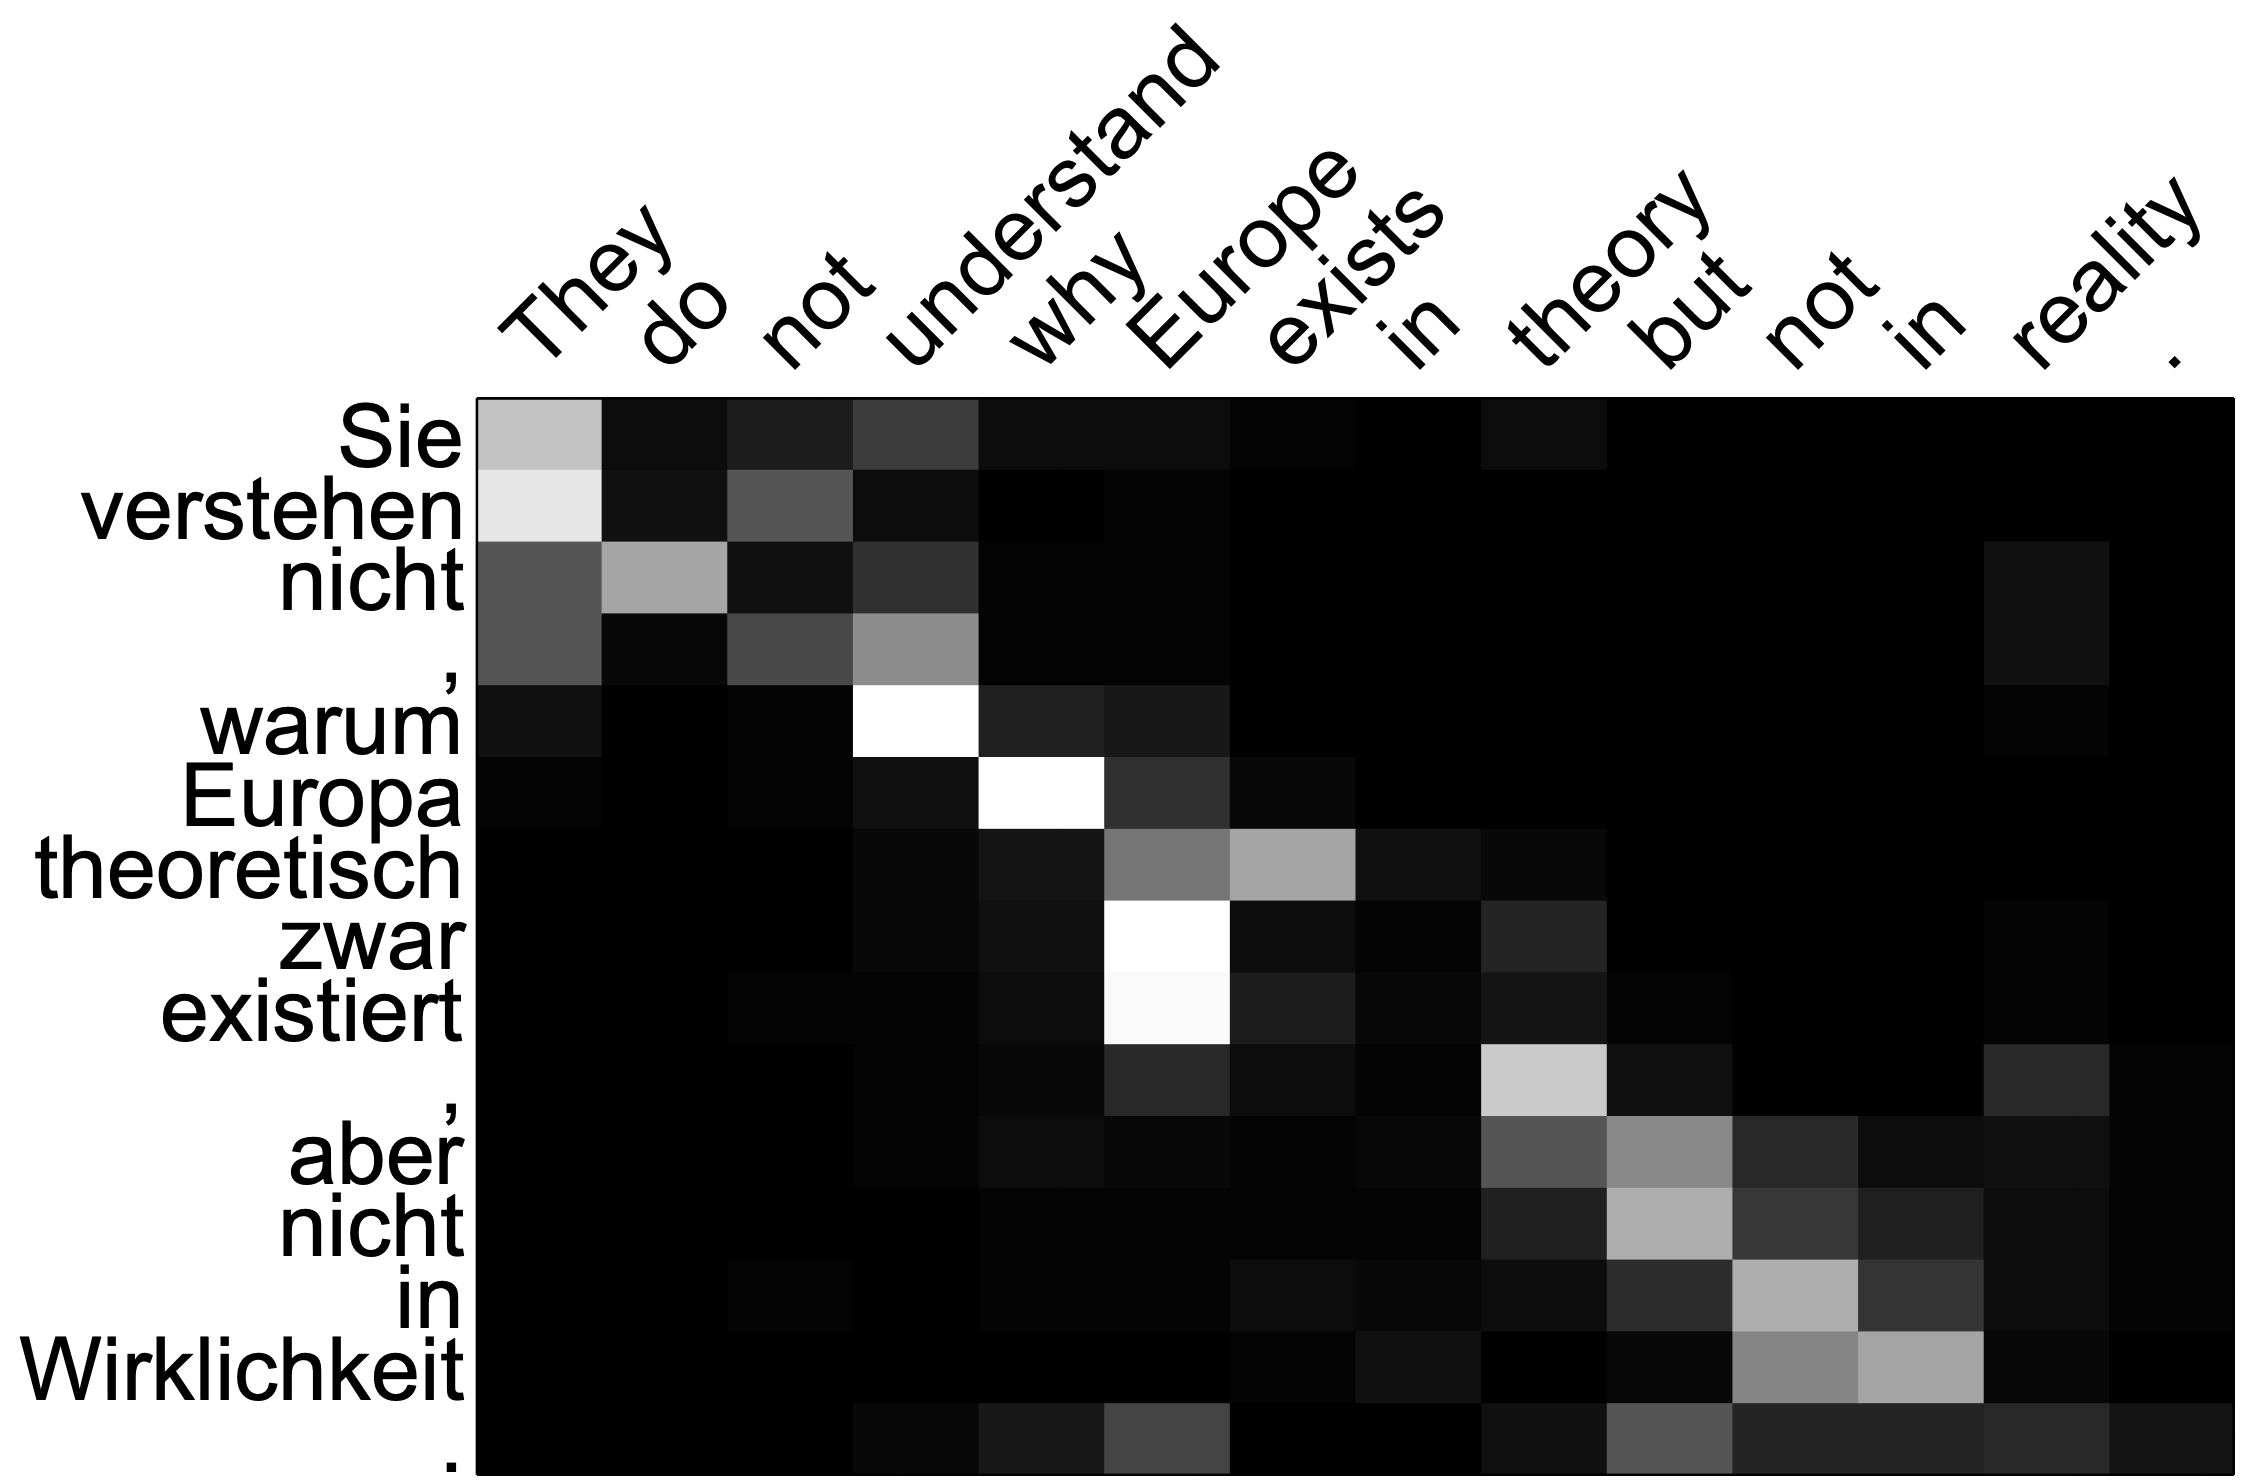
\includegraphics[width=0.95\textwidth]{assets/local_m}
      \caption{Local-M}
    \end{figure}
    \vspace{-7mm}
    \begin{figure}
      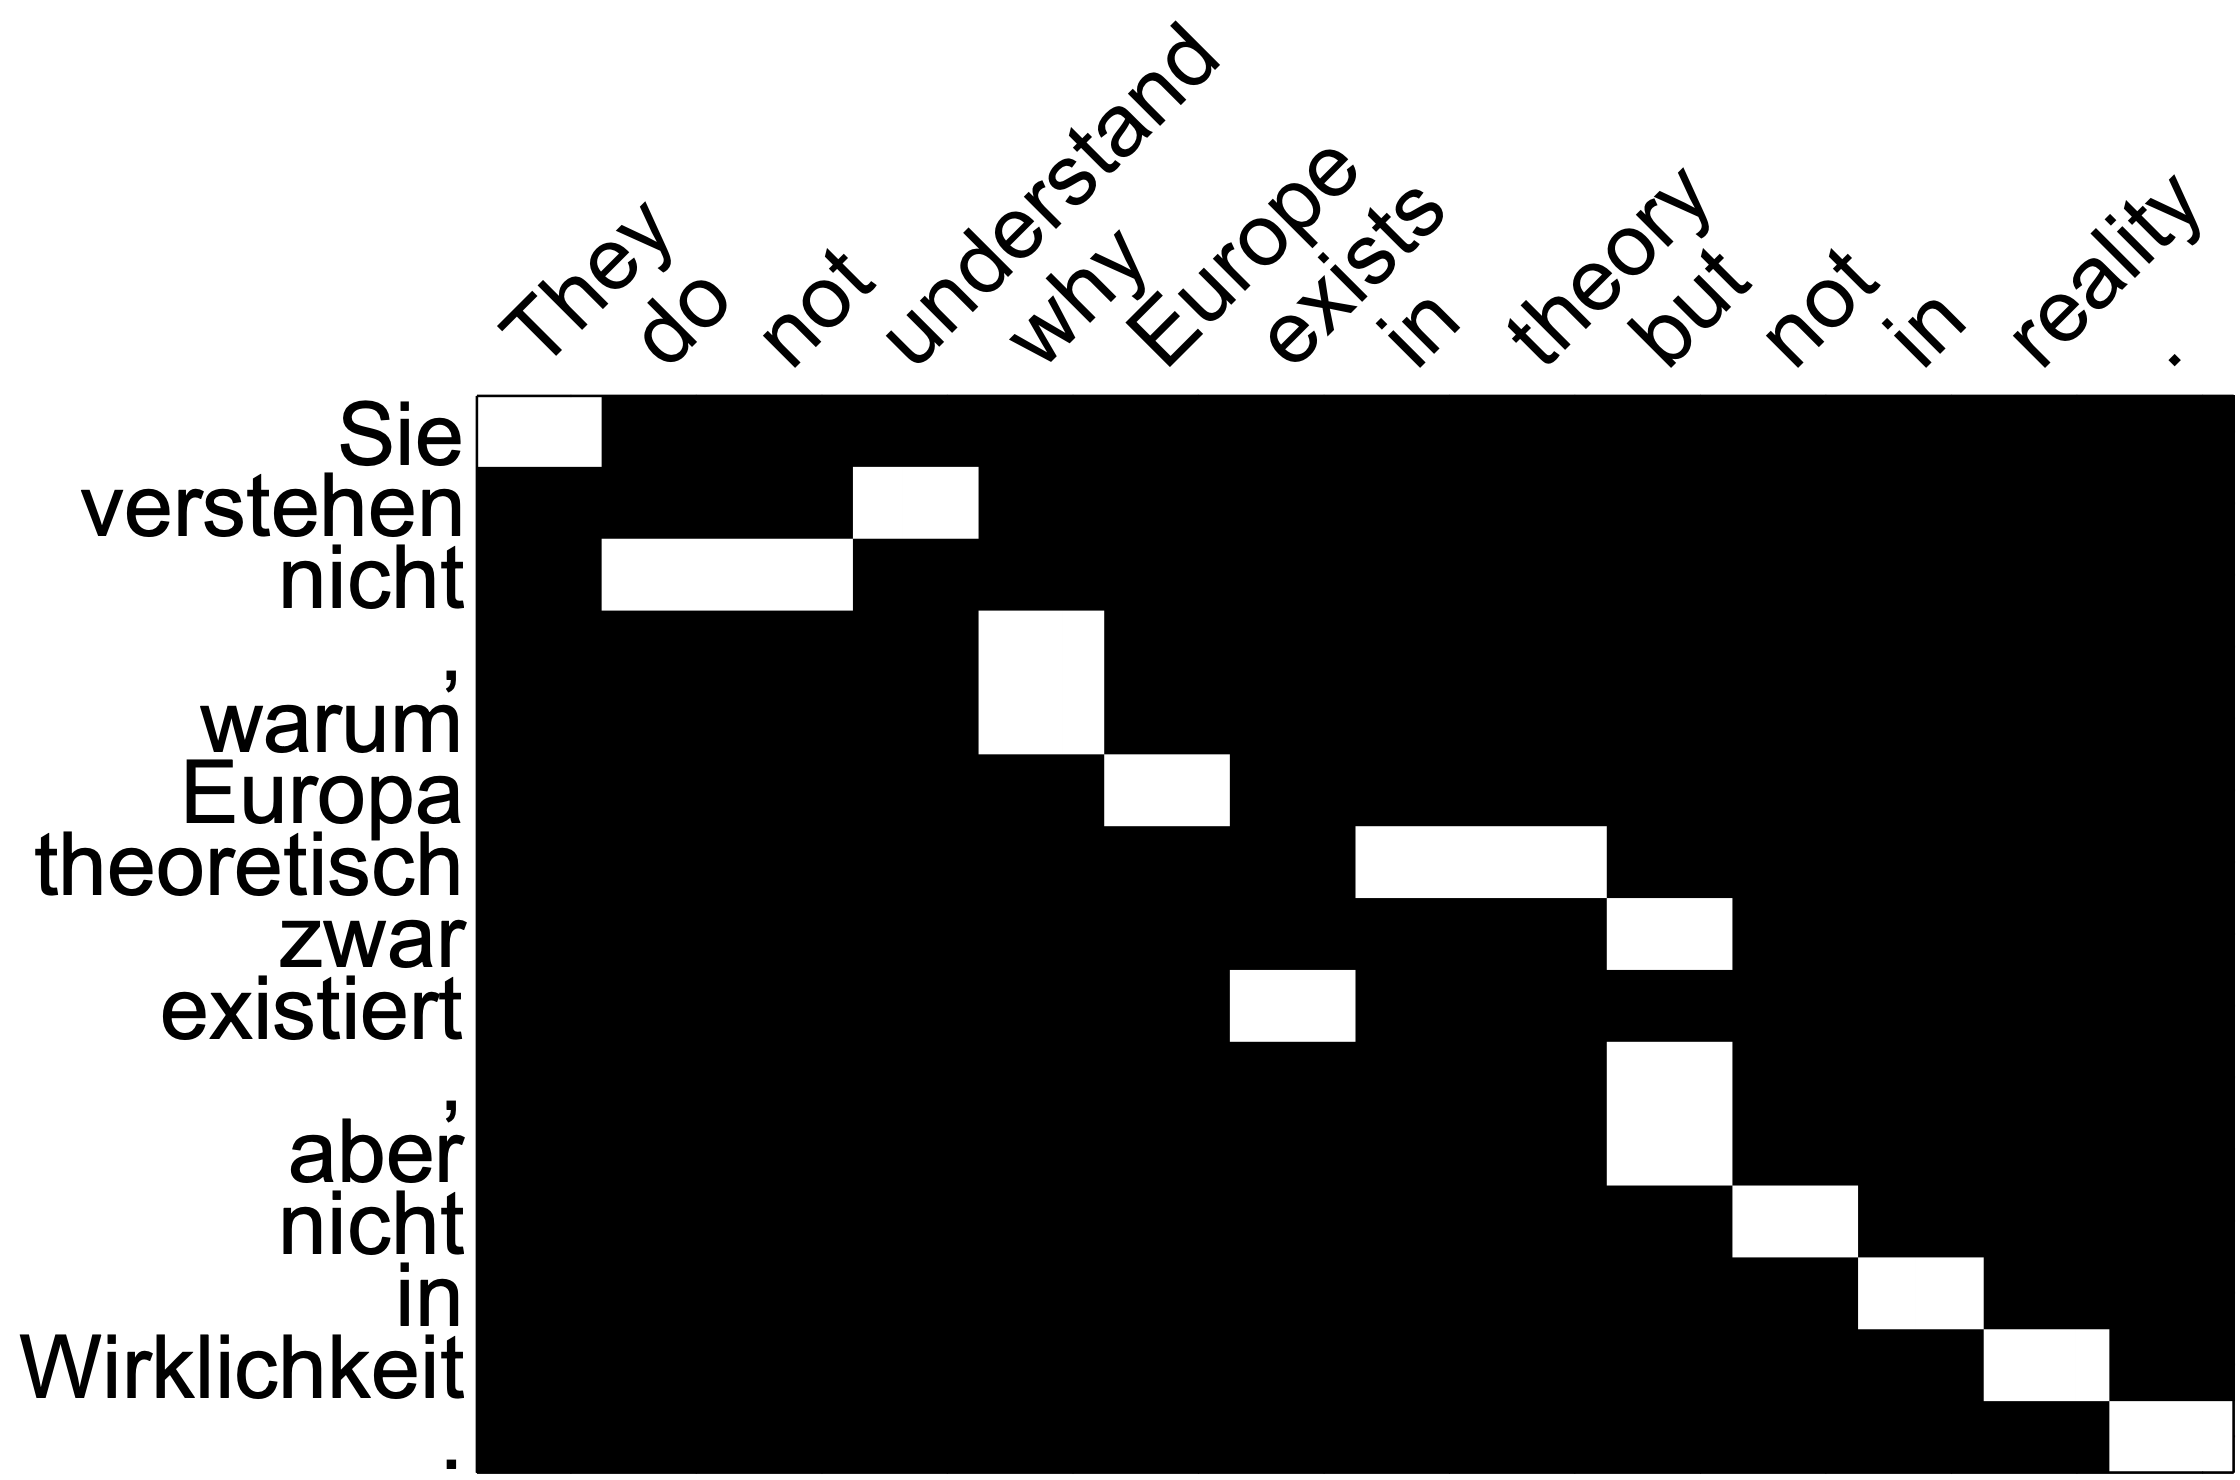
\includegraphics[width=0.95\textwidth]{assets/gold}
      \caption{Gold Alignments}
    \end{figure}
    \end{column}

  \end{columns}
\end{frame}

\begin{frame}
\frametitle{Fine-Grained Attention}
\begin{equation*}
  a^k \left( s_{i-1}, h_j \right) = \texttt{FF}^k(s_{i-1}, h_j)
\end{equation*}
\begin{equation*}
  \alpha_{ij}^d = \frac{\exp\left(a^d\left(s_{i-1}, h_j\right)\right)}{\sum_k \exp \left( a^d \left(s_{i-1}, h_k\right) \right)}
\end{equation*}
\begin{equation*}
  c_i = \sum_j \alpha_{ij} \odot h_j
\end{equation*}
\begin{itemize}
  \item What's different?
  \item Instead of a scalar scoring function, have it output a weight \textit{per} dimension
  \item Now a weighted average on the feature dimension \textit{instead} of the entire encoding
\end{itemize}
\end{frame}

\begin{frame}
  \frametitle{Fine-Grained Attention}
  \begin{equation*}
    c_i = \textcolor{BrickRed}{0.64} \cdot \begin{bmatrix*}[r] 0.17 \\ 0.53 \\ -0.22 \end{bmatrix*} + \textcolor{BrickRed}{0.12} \cdot \begin{bmatrix*}[r] 1.34 \\ 0.39 \\ 0.45 \end{bmatrix*} + \textcolor{BrickRed}{0.24} \cdot \begin{bmatrix*}[r] -0.08 \\ -1.39 \\ 1.21 \end{bmatrix*}
  \end{equation*}
  \vspace{1.5cm}
  \begin{equation*}
    c_i = \begin{bmatrix} \textcolor{WildStrawberry}{0.59} \\ \textcolor{Fuchsia}{0.18} \\ \textcolor{ForestGreen}{0.16} \end{bmatrix} \odot \begin{bmatrix*}[r] 0.17 \\ 0.53 \\ -0.22 \end{bmatrix*} + \begin{bmatrix} \textcolor{WildStrawberry}{0.09} \\ \textcolor{Fuchsia}{0.36} \\ \textcolor{ForestGreen}{0.74} \end{bmatrix} \odot \begin{bmatrix*}[r] 1.34 \\ 0.39 \\ 0.45 \end{bmatrix*} + \begin{bmatrix} \textcolor{WildStrawberry}{0.32} \\ \textcolor{Fuchsia}{0.46} \\ \textcolor{ForestGreen}{0.10} \end{bmatrix} \odot \begin{bmatrix*}[r] -0.08 \\ -1.39 \\ 1.21 \end{bmatrix*}
  \end{equation*}
\end{frame}

\begin{frame}
\frametitle{Multi-Headed Attention}
\begin{equation*}
  \alpha_{ij}^k = \frac{\exp\left(a^k\left(s_{i-1}, h_j\right)\right)}{\sum_k \exp \left( a^k \left(s_{i-1}, h_k\right) \right)}
\end{equation*}
\begin{itemize}
  \item Why not have $K$ attention weights?
\end{itemize}
\begin{equation*}
  c_i^{k} = \sum_j \alpha_{ij}^k \cdot h_j
\end{equation*}
\begin{equation*}
  c_i =\frac{1}{K} \sum_k c_i^k
\end{equation*}
\begin{itemize}
  \item \textit{Multi-Headed Attention} is just aggregating several attended representations of the encodings
  \item Fancy way of ensembling attention mechanisms
\end{itemize}
\end{frame}

\begin{frame}
  \frametitle{Multi-Headed Attention}
  \begin{equation*}
    \alpha_{ij}^d = \frac{\exp\left(a^d\left(s_{i-1}, h_j\right)\right)}{\sum_k \exp \left( a^d \left(s_{i-1}, h_k\right) \right)}
  \end{equation*}
  \begin{equation*}
    c_i^{k} = \sum_j \alpha_{ij}^k \cdot h_j
  \end{equation*}
  \begin{equation*}
    c_i = \begin{bmatrix*} c^0_{i} \\ \vdots \\ c^k_{i} \\ \vdots \\ c^K_{i} \end{bmatrix*} W_a
  \end{equation*}
  \begin{itemize}
    \item \textbf{Alternative:} Concat each context vector and use a linear layer to reduce the dimensionality
    \item Weighted Average of $K$ 'attended' context vectors!
  \end{itemize}
\end{frame}

\begin{frame}
  \frametitle{Multi-Headed Attention}
  \begin{figure}
      \centering
      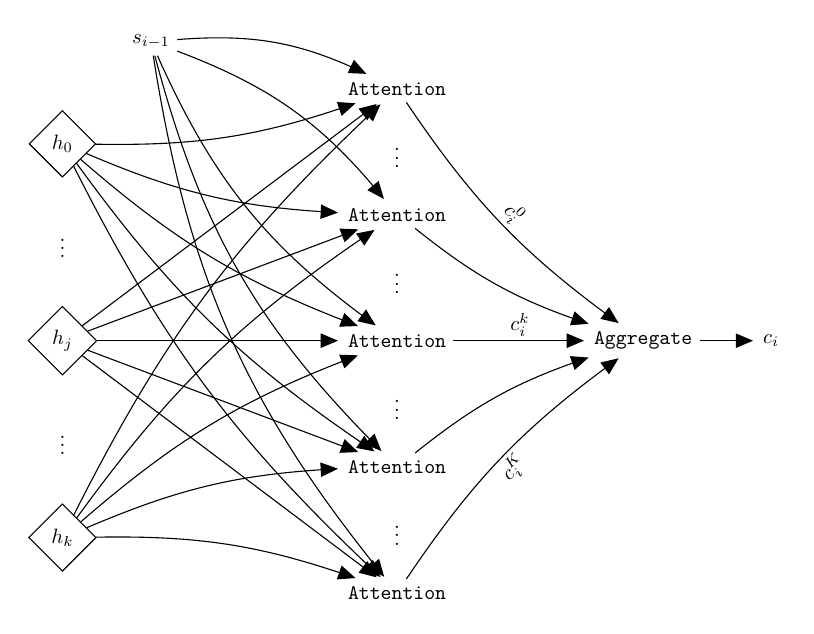
\begin{tikzpicture}[shorten >=1pt,node distance=1.25cm,on grid,auto, every node/.style={scale=0.75},
        el/.style={inner sep=2pt, align=left, sloped}]

        \node[draw,diamond]  (h2)  {$h_j$};
        \node[]  (h1) [above=of h2] {$\vdots$};
        \node[]  (h3) [below=of h2] {$\vdots$};
        \node[draw,diamond] [above=of h1]  (h0)  {$h_0$};
        \node[draw,diamond]  (h4) [below=of h3] {$h_{k}$};


        \node[] (a0) [right=of h2, xshift=4cm] {$\texttt{Attention}$};
        \node[] (tmp1) [above=of a0, yshift=-6mm] {$\vdots$};
        \node[] (a1) [above=of tmp1, yshift=-6mm] {$\texttt{Attention}$};
        \node[] (tmp2) [below=of a0, yshift=6mm] {$\vdots$};
        \node[] (a2) [below=of tmp2, yshift=6mm] {$\texttt{Attention}$};

        \node[] (tmp3) [above=of a1, yshift=-6mm] {$\vdots$};
        \node[] (tmp4) [below=of a2, yshift=6mm] {$\vdots$};
        \node[] (a3) [above=of tmp3, yshift=-6mm] {$\texttt{Attention}$};
        \node[] (a4) [below=of tmp4, yshift=6mm] {$\texttt{Attention}$};

        \node[] (s) [left=of a3, xshift=-2.5cm, yshift=8mm] {$s_{i-1}$};



        \node[] (agg) [right=of a0, xshift=2.5cm] {$\texttt{Aggregate}$};

        \node[] (c) [right=of agg, xshift=0.5cm] {$c_i$};

        \path[->]
          (h0) edge [bend right=10] node[] {} (a0)
          (h2) edge [] node[] {} (a0)
          (h4) edge [bend left=10] node[] {} (a0)
          (h0) edge [bend right=10] node[] {} (a1)
          (h2) edge [] node[] {} (a1)
          (h4) edge [bend left=10] node[] {} (a1)
          (h0) edge [bend right=10] node[] {} (a2)
          (h2) edge [] node[] {} (a2)
          (h4) edge [bend left=10] node[] {} (a2)
          (h0) edge [bend right=10] node[] {} (a3)
          (h2) edge [] node[] {} (a3)
          (h4) edge [bend left=10] node[] {} (a3)
          (h0) edge [bend right=10] node[] {} (a4)
          (h2) edge [] node[] {} (a4)
          (h4) edge [bend left=10] node[] {} (a4)

          (s) edge [bend right=15] node[] {} (a0)
          (s) edge [bend left=15] node[] {} (a1)
          (s) edge [bend right=15] node[] {} (a2)
          (s) edge [bend left=15] node[] {} (a3)
          (s) edge [bend right=15] node[] {} (a4)

          (a0) edge [] node[el] {$c_{i}^k$} (agg)
          (a1) edge [bend right=10] node[] {} (agg)
          (a2) edge [bend left=10] node[] {} (agg)
          (a3) edge [bend right=10] node[el, above] {$c_{i}^0$} (agg)
          (a4) edge [bend left=10] node[el, below] {$c_{i}^K$} (agg)

          (agg) edge [] node[] {} (c);

      \end{tikzpicture}
    \end{figure}
\end{frame}

% \begin{frame}
%   \frametitle{MHA Visual from the Paper}
%
% \end{frame}

\begin{frame}
  \frametitle{Self-Attention: Generalized}
  \begin{equation*}
    \texttt{Attention}\left(Q, K, V \right) = \texttt{softmax}\left(\frac{QK^T}{\sqrt{d_k}}\right) V
  \end{equation*}
  \begin{itemize}
    \item Query $Q$, Key $K$, and Value $V$
    \item $d_k$ is the dimensionality of the query and keys
    \item \textbf{Note} that this implies that we can re-mix the encodings via linear layers before attending
    \item \textbf{Note} the similiarity to Luong's Scaled Dot Attention
  \end{itemize}
\end{frame}

% MESSY
\begin{frame}
  \frametitle{Self-Attention: What are Queries, Keys, and Values?}
  % \begin{itemize}
  %   \item \textbf{Encoders}
  %   \begin{itemize}
  %     \item Source Embeddings, optionally re-mixed with linear layers
  %   \end{itemize}
  % \end{itemize}
  % \begin{itemize}
  %   \item \textbf{Decoders}
  %   \begin{itemize}
  %     \item More complicated...
  %     \item Technically 2 Self-Attentions
  %     \item One that is the decoded embeddings
  %     \item Then use that as the value for a second attention
  %   \end{itemize}
  % \end{itemize}
\end{frame}

\begin{frame}
  \frametitle{Self-Attention: Packing the Encodings}
  \begin{itemize}
    \item To create Queries, Keys, and Values, we must pack the encodings
    \item Create a matrix $H \in \mathbb{R}^{S \times d}$
    \item $S$ is sequence length, $d$ is the dimensionality of the vectors
  \end{itemize}
  \begin{equation*}
    H = \begin{bmatrix}
    \longleftarrow h_0 \longrightarrow \\
    \vdots \\
    \longleftarrow h_j \longrightarrow  \\
    \vdots \\
    \longleftarrow h_k \longrightarrow
\end{bmatrix}
  \end{equation*}
\end{frame}

\begin{frame}
  \frametitle{Self-Attention: Computation Graph}
  \begin{figure}
      \centering
      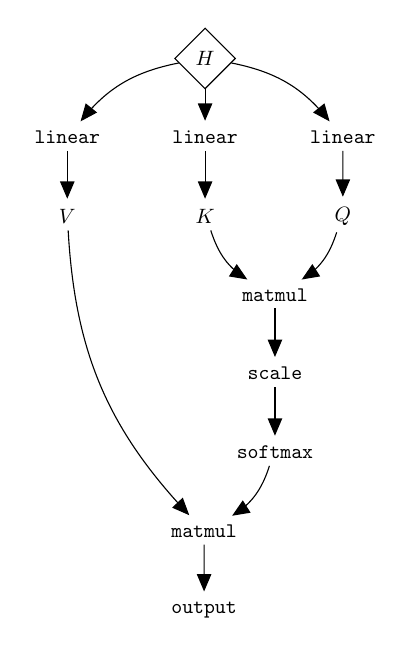
\begin{tikzpicture}[shorten >=1pt,node distance=1cm,on grid,auto, every node/.style={scale=0.75},
        el/.style={inner sep=2pt, align=left, sloped}]

        \node[draw,diamond]  (H)  {$H$};

        \node[] (WK) [below=of H] {$\texttt{linear}$};
        \node[] (WQ) [right=of WK, xshift=1cm] {$\texttt{linear}$};
        \node[] (WV) [left=of WK, xshift=-1cm] {$\texttt{linear}$};

        \node[] (Q) [below=of WQ] {$Q$};
        \node[] (K) [below=of WK] {$K$};
        \node[] (V) [below=of WV] {$V$};

        \node[] (matmul) [below=of Q, xshift=-1.15cm] {$\texttt{matmul}$};
        \node[] (scale) [below=of matmul] {$\texttt{scale}$};
        \node[] (softmax) [below=of scale] {$\texttt{softmax}$};
        \node[] (matmul2) [below=of softmax, xshift=-1.2cm] {$\texttt{matmul}$};

        \node[] (c) [below=of matmul2] {$\texttt{output}$};


        \path[->]
        (H) edge [bend left=20] node[] {} (WQ)
        (H) edge [] node[] {} (WK)
        (H) edge [bend right=20] node[] {} (WV)

        (WQ) edge [] node[] {} (Q)
        (WK) edge [] node[] {} (K)
        (WV) edge [] node[] {} (V)

        (Q) edge [bend left=20] node[] {} (matmul)
        (K) edge [bend right=20] node[] {} (matmul)
        (matmul) edge [] node[] {} (scale)
        (scale) edge [] node[] {} (softmax)
        (softmax) edge [bend left=20] node[] {} (matmul2)
        (V) edge [bend right=20] node[] {} (matmul2)
        (matmul2) edge [] node[] {} (c);

      \end{tikzpicture}
    \end{figure}
\end{frame}


\section{Practical Considerations}
% Rework
\begin{frame}
\frametitle{Masking}

\end{frame}

\begin{frame}
\frametitle{Which one to use?}
\begin{itemize}
  \item Trend seems to be moving towards \textbf{Transformers}
  \item AKA a series of Self-Attentions inside Multi-headed Attentions
  \item Ideally, experiment and go crazy
\end{itemize}
\end{frame}

\begin{frame}
\frametitle{Mixing and Matching}
  \begin{itemize}
    \item Remember! You can always mix and match!
    \item Different attention mechanisms under MHA
    \item Etc, etc
  \end{itemize}
\end{frame}

%%%%%%%%%%%%%%%%%%%%%%%%%%%%%%%%%%%%%%%%%%%%%%%%%%%%%%%%%%%%%%%%%%%%%%%%%%%%%%%%

\section{Tools, References, and Further Reading}


\begin{frame}
\frametitle{Papers}
  \begin{itemize}
    \item \href{https://arxiv.org/pdf/1409.0473}{Bahdanau et al., Neural Machine Translation by Jointly Learning to Align and Translate}
    \item \href{https://arxiv.org/pdf/1508.04025}{Luong et al.m Effective Approaches to Attention-based Neural Machine Translation}
    \item \href{https://papers.nips.cc/paper/7181-attention-is-all-you-need.pdf}{Vaswani et al., Attention is All You Need}
    \item \href{http://www.aclweb.org/anthology/N13-1073}{Dyer et al., A Simple, Fast, and Effective Reparameterization of IBM Model 2}
  \end{itemize}
\end{frame}


% Refs, ideas, etc


\end{document}
